\documentclass[aps,prb,reprint,superscriptaddress,nofootinbib,longbibliography,floatfix]{revtex4-2}

\usepackage[utf8]{inputenc}
\usepackage[T1]{fontenc}
\usepackage{lmodern}
\usepackage{amsmath,amssymb}
\usepackage{bm}
\usepackage{graphicx}
\usepackage{xcolor}
\usepackage{algorithm}      % algorithm boxes must use [H] in REVTeX
\usepackage{algpseudocode}
\usepackage[colorlinks=true,linkcolor=blue!55!black,citecolor=blue!55!black,urlcolor=blue!55!black]{hyperref}

\graphicspath{{figures/}}

\renewcommand{\topfraction}{0.9}
\renewcommand{\dbltopfraction}{0.9}
\renewcommand{\bottomfraction}{0.8}
\renewcommand{\textfraction}{0.07}
\renewcommand{\floatpagefraction}{0.75}
\renewcommand{\dblfloatpagefraction}{0.75}
\setcounter{topnumber}{3}
\setcounter{dbltopnumber}{3}
\setcounter{bottomnumber}{2}
\setcounter{totalnumber}{5}

\newcommand{\E}{\mathbb{E}}
\newcommand{\vtheta}{\bm{\theta}}
\newcommand{\vX}{\bm{X}}
\newcommand{\vy}{\bm{y}}
\newcommand{\MSE}{\mathrm{MSE}}

\begin{document}

\title{Polynomial regression of the Runge function: generalization, resampling and optimization}

\author{Rasul Ruslanovitsj {\O}zdber}
\affiliation{Department of Physics, University of Oslo, Norway}
\date{October 5, 2026}

\begin{abstract}
We study polynomial regression of the Runge function using ordinary least squares, Ridge and Lasso. The known target makes it possible to examine prediction error and the bias--variance trade-off while separately checking numerical optimization. We vary polynomial degree, sample size and noise, compare bootstrap estimates with cross-validation, and test gradient methods against reference solutions. For 100 observations with noise standard deviation 0.1, ten-fold cross-validation selects degree-12 ordinary least squares, with MSE 0.0113 on 2000 independent observations. Ridge gives nearly the same selected fit but substantially stabilizes higher-degree models. Bootstrap estimates from a small training sample are sensitive to missing boundary observations, and mean and median errors can favor different degrees. At degree six, plain gradient descent at the Hessian-based rate takes 14,399 iterations to reach the specified coefficient tolerance, while the best tested momentum rate takes 656. These results show why model selection, prediction accuracy and optimizer convergence must be assessed with distinct criteria.
\end{abstract}

\maketitle

\section{Introduction}\label{sec:intro}
\emph{LLM contribution: the abstract and this section were drafted with assistance; see Appendix~\ref{app:llm}.}

Polynomial regression provides a direct way to study how model complexity affects prediction. Increasing the degree gives the model more freedom, but also makes it easier to fit noise and produces increasingly correlated columns in the design matrix. The Runge function is useful here because its central peak is not well described by a very low-degree polynomial, while its exact value is known everywhere in the chosen interval. Following the project specification, this allows us to compare fitted predictions both with noisy observations and with the underlying function \cite{Project1_2026}.

The project asks three related questions. First, how do polynomial degree, sample size and noise affect the quality of OLS, Ridge and Lasso fits? Second, what do bootstrap and cross-validation tell us about choosing a model, and when do their estimates disagree? Third, how do the learning rate, optimizer and batch size affect convergence to a reference solution? These questions follow the regression, resampling and optimization material from weeks 35--38 \cite{HjorthJensen2026,HjorthJensen2026exercises}.

We separate the statistical and numerical comparisons. A low training objective does not guarantee low test error, and a low test error does not require coefficients to match an optimum very accurately. OLS and Ridge give closed-form reference solutions for testing iterative methods. For Lasso, Scikit-Learn's coordinate-descent solution provides a reference, while custom subgradient methods address the optimization question in part g. Additional proximal methods and known-function experiments are identified as supplementary checks rather than required course algorithms.

Section~\ref{sec:theory} defines the models and evaluation procedures. Section~\ref{sec:implementation} describes the implementation and checks. Section~\ref{sec:results} follows parts a--i of the project, and Section~\ref{sec:conclusion} discusses the main findings and limitations. Code and saved numerical results are available at \url{https://github.com/rasuluzd/fys-stk3155-project1}. Appendix~\ref{app:llm} records the use of LLMs.

\section{Theory and methods}\label{sec:theory}
\emph{LLM contribution: this section was drafted with assistance; see Appendix~\ref{app:llm}.}

\subsection{Data and model}\label{sec:data}
The data model and degree sweep follow Project~1a and the polynomial-regression exercises
\cite{Project1_2026,HjorthJensen2026exercises}. The design matrix contains powers of the input;
the model is nonlinear in $x$ but linear in its fitted coefficients.
\begin{equation}
f(x)=\frac{1}{1+25x^2},\qquad x\in[-1,1]. \label{eq:runge}
\end{equation}
\begin{equation}
y_i=f(x_i)+\varepsilon_i,\qquad \varepsilon_i\sim\mathcal N(0,\sigma^2), \label{eq:data}
\end{equation}
% Evidence: code/settings.py, regression.make_data, part_a.json/main.
Unless specified otherwise, $N=100$ inputs are drawn independently and uniformly from $[-1,1]$,
with $\sigma=0.1$ and an 80/20 train/test split. Random inputs are allowed by the project and
let us study sensitivity to input locations as well as noise. Later CV and independent test evaluation supplement this small holdout. Seed 2026 fixes
this baseline; repeated-dataset experiments use separate seeds. The unregularized main fit includes
degrees 0--15, while the broader sensitivity and model-selection experiments extend to degree 20.
\begin{equation}
\tilde y(x)=\beta_0+\sum_{j=1}^{p}\beta_j x^j . \label{eq:model}
\end{equation}
The degree counts slopes; an intercept is fitted in addition. A constant model has degree zero.
The even target favors even powers in the population, but an asymmetric finite sample can give
nonzero odd slopes.

\subsection{Scaling and the intercept}\label{sec:scaling}
For degree $p$, the raw feature matrix is $A_{ij}=x_i^j$ for $j=1,\ldots,p$. On each training set of size $n$, we compute
\begin{align}
\mu_j&=\frac1n\sum_i A_{ij},&
s_j^2&=\frac1n\sum_i(A_{ij}-\mu_j)^2,\nonumber\\
X_{ij}&=\frac{A_{ij}-\mu_j}{s_j},&
y_{c,i}&=y_i-\bar y_{\rm train}.
\end{align}
Centering the features and target handles the intercept without adding a penalized constant column. Dividing by $s_j$ puts slopes on comparable scales for the penalty. The fitted prediction and original coefficients are
\begin{align}
\tilde y(x)&=\bar y_{\rm train}+\sum_{j=1}^p\theta_j\frac{x^j-\mu_j}{s_j},\nonumber\\
\beta_j&=\theta_j/s_j,\qquad
\beta_0=\bar y_{\rm train}-\sum_j\beta_j\mu_j .
\end{align}
The raw intercept is therefore generally different from $\bar y_{\rm train}$. We reuse the training means and scales on held-out observations. Refitting these values on the test set would change the coordinate system, while estimating them from all observations would let held-out inputs influence fitting. Scaling reduces differences in column magnitude but does not remove correlations among powers. In exact arithmetic, invertible scaling preserves full-rank OLS predictions with an intercept; it changes Ridge and Lasso at fixed $\lambda$ because their coefficient penalties depend on the chosen coordinates.
The implemented preprocessing follows the centering and scaling procedure in
\cite[Sec.~3.13]{HjorthJensen2026} and Week~37, Exercise~1
\cite{HjorthJensen2026exercises}. In the following cost functions, $\vX$ denotes the training-standardized design matrix,
$\vy$ the centered target, and $\vtheta$ the standardized slope coefficients.

\subsection{Ordinary least squares}
The least-squares objective and pseudoinverse solution follow
\cite[Secs.~3.1--3.3]{HjorthJensen2026}. The implementation uses
\texttt{numpy.linalg.pinv}, as permitted in Project~1a, rather than explicitly inverting
$\vX^T\vX$; this avoids squaring the condition number in the numerical solve.
\begin{equation}
C(\vtheta)=\frac1n\|\vy-\vX\vtheta\|_2^2, \label{eq:ols_cost}
\end{equation}
\begin{equation}
\hat{\vtheta}_{\rm OLS}=\vX^+\vy=\sum_{j:d_j>0}\frac{\bm u_j^T\vy}{d_j}\,\bm v_j . \label{eq:ols_svd}
\end{equation}
Differentiating Eq.~(\ref{eq:ols_cost}) and setting the result to zero gives
$\vX^T\vX\hat{\vtheta}=\vX^T\vy$. Writing $\vX=UDV^T$ gives Eq.~(\ref{eq:ols_svd}).
In floating-point calculations the pseudoinverse uses a relative singular-value cutoff of
$10^{-15}$. For fixed full-rank inputs and independent noise, the coefficient variance in
singular direction $j$ is $\sigma^2/d_j^2$. Thus the SVD solve avoids an unnecessarily unstable
matrix inversion but cannot remove sensitivity already present in the fitted model.

\subsection{Ridge regression}
Ridge adds a squared penalty to the standardized slopes, with the intercept left unpenalized
\cite[Secs.~3.8 and 3.13]{HjorthJensen2026}. This report uses mean squared loss, as in
Week~37, Exercise~2. Consequently the linear system contains $n\lambda\bm I$ and the
equivalent Scikit-Learn setting is $\alpha=n\lambda$
\cite[Eq.~(3.95)]{HjorthJensen2026}. Earlier examples that use a sum of squared residuals
absorb this factor of $n$ into their penalty parameter.
\begin{equation}
C(\vtheta)=\frac1n\|\vy-\vX\vtheta\|_2^2+\lambda\|\vtheta\|_2^2, \label{eq:ridge_cost}
\end{equation}
\begin{align}
\hat{\vtheta}_{\rm Ridge}&=(\vX^T\vX+n\lambda\bm I)^{-1}\vX^T\vy\nonumber\\
&=\sum_{j=1}^{p}\frac{d_j}{d_j^2+n\lambda}\,(\bm u_j^T\vy)\,\bm v_j,\qquad \lambda>0. \label{eq:ridge}
\end{align}
Relative to OLS, direction $j$ is multiplied by
$q_j=d_j^2/(d_j^2+n\lambda)$. This suppresses small singular directions most strongly.
The effective slope degrees of freedom are $\sum_j q_j$; the unpenalized intercept adds one \cite[Sec.~1.22]{HjorthJensen2026}.
At large $\lambda$, predictions approach the training mean. This lowers flexibility and can
reduce variance, but the resulting bias can increase prediction error. The degree and penalty
therefore both need to be assessed.

\subsection{Lasso regression}
The absolute-value penalty follows the course treatment of Lasso
\cite[Secs.~3.9--3.10]{HjorthJensen2026}. The conditions below say that an active
coefficient balances the residual correlation against its penalty, while a zero coefficient
allows that correlation to lie within an interval. They provide a numerical check of a
computed solution. With the present loss convention, Scikit-Learn uses $\alpha=\lambda/2$.
\begin{equation}
C(\vtheta)=\frac1n\|\vy-\vX\vtheta\|_2^2+\lambda\|\vtheta\|_1 , \label{eq:lasso_cost}
\end{equation}
\begin{equation}
\frac2n\bm x_j^T(\vy-\vX\hat{\vtheta})\in
\begin{cases}\{\lambda\,\mathrm{sign}(\hat\theta_j)\}, & \hat\theta_j\neq0,\\ [-\lambda,\lambda], & \hat\theta_j=0.\end{cases}
\label{eq:kkt}
\end{equation}
At zero, the subdifferential of $|\theta_j|$ is $[-1,1]$; away from zero it is its sign.
There is no OLS-like closed form for a general correlated design. In particular,
all slopes are zero when $\lambda\geq\|(2/n)\vX^T\vy\|_\infty$. Lasso can therefore select
a sparse model, although highly correlated powers can substitute for one another and make the
individual selected terms unstable.

\subsection{Error measures}
MSE and $R^2$ are the regression measures introduced in
\cite[Sec.~3.5]{HjorthJensen2026} and Week~35, Exercise~2.
In Eq.~(\ref{eq:metrics}), $n$ denotes the number of observations in the set being scored,
and $\bar y$ is the mean target in that set. A finite test MSE can fall below $\sigma^2$;
the irreducible-noise bound applies to expected risk.
\begin{equation}
\MSE=\frac1n\sum_{i}(y_i-\tilde y_i)^2,\qquad R^2=1-\frac{\sum_i(y_i-\tilde y_i)^2}{\sum_i(y_i-\bar y)^2}. \label{eq:metrics}
\end{equation}
On a fixed evaluation set, $R^2=1-\MSE/\operatorname{Var}_n(y)$, where the variance uses
divisor $n$, so the two measures rank models in opposite order. A negative $R^2$ means the
predictions are worse than the constant mean of that evaluation set.

\subsection{The bias--variance decomposition}\label{sec:biasvar_theory}
The decomposition follows the course derivation
\cite[Sec.~2.10, Eq.~(2.52)]{HjorthJensen2026}. The expectation averages over the random
training data and independent test noise; the function $f$ and the $n_t$ evaluation inputs
are held fixed. Week~36, Exercise~2 makes these sources of randomness explicit
\cite{HjorthJensen2026exercises}.
Let $D$ denote the random training set and let $g_D(x)$ be the fitted prediction at a fixed input. Define $m(x)=\E_D[g_D(x)]$. An independent test observation is $Y=f(x)+\varepsilon$, with $\E[\varepsilon]=0$ and $\E[\varepsilon^2]=\sigma^2$. Adding and subtracting $m(x)$ gives
\[
Y-g_D(x)=(f(x)-m(x))+(m(x)-g_D(x))+\varepsilon.
\]
Squaring produces three squared terms and three cross terms. The cross term between $f-m$ and $m-g_D$ vanishes because $\E_D[m-g_D]=0$. The term involving $(f-m)\varepsilon$ vanishes because the test noise has mean zero. Independence of training data and test noise removes the remaining cross term. Hence
\[
\E_{D,\varepsilon}[(Y-g_D(x))^2]
=(f(x)-m(x))^2+\E_D[(g_D(x)-m(x))^2]+\sigma^2.
\]
Averaging over the fixed evaluation inputs gives Eq.~(\ref{eq:biasvar}). Bias is the systematic difference between the mean fitted function and $f$; variance measures changes between training sets at the same input. The noise term concerns a fresh response. Gaussian noise is used in the experiments, but the identity only requires the stated means, variances and independence. Since the training inputs are redrawn in the independent-dataset experiments, their randomness is part of $D$, along with the training noise.
\begin{align}
\frac1{n_t}\sum_i\E\big[(y_i-\tilde y_i)^2\big]={}&\underbrace{\frac1{n_t}\sum_i\big(f_i-\E[\tilde y_i]\big)^2}_{\mathrm{Bias}^2[\tilde y]}\nonumber\\
&+\underbrace{\frac1{n_t}\sum_i\E\big[(\tilde y_i-\E[\tilde y_i])^2\big]}_{\mathrm{Var}[\tilde y]}+\,\sigma^2. \label{eq:biasvar}
\end{align}

\subsection{Resampling: the bootstrap and cross-validation}\label{sec:resampling}
The bootstrap replaces an unknown training-data distribution by its empirical distribution. We draw paired observations with replacement from the training set and fit a new model to each draw, keeping the test observations fixed. After $n$ draws, the expected number of distinct training observations is $n[1-(1-1/n)^n]$, approximately $0.632n$. A resample can therefore lose important boundary coverage even though it still contains $n$ rows. Algorithm~\ref{alg:bootstrap} implements this procedure.

There is a useful finite-sample distinction. At test input $i$, let $g_{bi}$ be bootstrap prediction $b$ and $\bar g_i=B^{-1}\sum_b g_{bi}$. With variance divisor $B$,
\begin{align}
\frac1{n_tB}\sum_{i,b}(y_i-g_{bi})^2
={}&\frac1{n_t}\sum_i(y_i-\bar g_i)^2\nonumber\\
&+\frac1{n_tB}\sum_{i,b}(g_{bi}-\bar g_i)^2 .
\end{align}
This is an exact identity for the stored predictions, because deviations from $\bar g_i$ sum to zero. It does not establish that the bootstrap accurately estimates population bias and variance. Replacing the known $f_i$ by noisy $y_i=f_i+\varepsilon_i$ changes the measured squared bias by
\[
\frac1{n_t}\sum_i\left[\varepsilon_i^2+
2\varepsilon_i(f_i-\bar g_i)\right].
\]
Its expectation over independent test noise is $\sigma^2$, but the realized difference includes a cross term.

In $k$-fold CV, each fold is predicted by a model fitted to the remaining folds. The mean held-out MSE is used to compare candidate degrees and penalties. The project requests both five and ten folds; for 100 observations these train on 80 and 90 observations, respectively. Candidates share the same fold assignments so their comparison does not also change which points are held out. Algorithm~\ref{alg:cv} includes preprocessing inside each fit.
The bootstrap and fold loops follow the procedures in
\cite[Secs.~2.11--2.12]{HjorthJensen2026} and Week~36, Exercises~3--4
\cite{HjorthJensen2026exercises}. Each fit learns its own preprocessing. The reported fold
standard error is descriptive because the training folds overlap. The one-standard-error
selection rule is the additional simplicity heuristic in
\cite[Sec.~3.14, Eq.~(3.96)]{HjorthJensen2026}.
For the joint degree--penalty search, the implementation defines simplicity by degree for OLS,
effective slope degrees of freedom for Ridge, and the number of nonzero slopes in the full-data
Lasso fit. Ties are broken by CV MSE. This extends the fixed-degree, largest-penalty convention
in the notes; it is a stated modeling choice rather than a new significance test.

\begin{algorithm}[H]
\caption{Bootstrap estimate of the bias--variance decomposition.}\label{alg:bootstrap}
\begin{algorithmic}[1]
\Require training set of $n$ points, $n_t$ test points $(x_j,y_j)$, $B$
\For{$b=1,\dots,B$}
  \State draw $n$ indices with replacement
  \State fit model (and scaler) to these $n$ points
  \State $\tilde y_j^{(b)}\gets$ prediction at every test input $x_j$
\EndFor
\State $\langle\tilde y_j\rangle\gets\frac1B\sum_b\tilde y_j^{(b)}$
\State error $\gets\frac{1}{n_t}\sum_j\frac1B\sum_b\big(y_j-\tilde y_j^{(b)}\big)^2$
\State bias$^2\gets\frac{1}{n_t}\sum_j\big(y_j-\langle\tilde y_j\rangle\big)^2$ \Comment{$y_j\to f(x_j)$: known-function estimate}
\State variance $\gets\frac{1}{n_t}\sum_j\frac1B\sum_b\big(\tilde y_j^{(b)}-\langle\tilde y_j\rangle\big)^2$
\end{algorithmic}
\end{algorithm}

\begin{algorithm}[H]
\caption{$k$-fold cross-validation with the scaling inside the loop.}\label{alg:cv}
\begin{algorithmic}[1]
\Require data $(\bm x,\vy)$, model, $k$
\State shuffle the indices and split them into folds $F_1,\dots,F_k$
\For{$l=1,\dots,k$}
  \State $\mathcal T\gets$ all points not in $F_l$
  \State compute $\bar x_j$, $s_j$, $\bar y$ on $\mathcal T$ only; scale $\mathcal T$ and $F_l$
  \State fit the model on $\mathcal T$, predict on $F_l$
  \State $\MSE_l\gets$ mean squared error on $F_l$
\EndFor
\State \Return $\mathrm{CV}=\frac1k\sum_l\MSE_l$, \; $\mathrm{SE}=\mathrm{sd}_{k-1}(\MSE_l)/\sqrt k$
\end{algorithmic}
\end{algorithm}

\subsection{Gradient descent}\label{sec:gd_theory}
The cost, gradient and update loop follow the three-function structure of Week~37,
Exercise~4 \cite{HjorthJensen2026exercises}. For Ridge, differentiating the mean-loss
objective gives
\begin{equation}
\nabla C(\vtheta)=\frac2n\vX^T(\vX\vtheta-\vy)+2\lambda\vtheta.
\end{equation}
Setting $\lambda=0$ gives OLS. The Hessian and fixed-rate stability analysis are those of
\cite[Secs.~4.3--4.5]{HjorthJensen2026}.
\begin{equation}
\vtheta_{k+1}=\vtheta_k-\eta\nabla C(\vtheta_k), \label{eq:gd}
\end{equation}
\begin{equation}
\bm H=\frac2n\vX^T\vX+2\lambda\bm I, \label{eq:hessian}
\end{equation}
For positive definite $\bm H$, with $e_{k,i}$ the coefficient error in eigenmode $i$,
\begin{equation}
e_{k,i}=(1-\eta h_i)^k\,e_{0,i},\qquad 0<\eta<\eta_{\max}=\frac{2}{h_{\max}}, \label{eq:gd_modes}
\end{equation}
The recurrence follows by subtracting the optimum from the quadratic update:
$e_{k+1}=(I-\eta H)e_k$. Diagonalizing $H$ separates the error into the factors shown above.
With $\kappa=h_{\max}/h_{\min}$, the best worst-case contraction factor is
$q=(\kappa-1)/(\kappa+1)$ \cite[Sec.~4.5]{HjorthJensen2026}. For large $\kappa$ this gives an
iteration scale proportional to $\kappa\log(1/\epsilon)$; the actual count also depends on
the starting error's projection onto each eigenvector. Singular OLS designs require separate
treatment of null directions.
The minimum worst-case contraction factor is obtained at
$\eta_*=2/(h_{\max}+h_{\min})$. The optional spectral comparison with early stopping
is kept in Appendix~\ref{app:additional_checks}.

\subsection{Momentum and adaptive learning rates}\label{sec:adaptive_theory}
Momentum follows Week~37, Exercise~6; AdaGrad, RMSprop and Adam follow Week~38,
Exercises~1--3 \cite{HjorthJensen2026exercises} and
\cite[Secs.~4.6 and 4.8--4.12]{HjorthJensen2026}. Unless otherwise stated, the code uses
$\beta=0.9$, $\rho=0.99$, $\beta_1=0.9$, $\beta_2=0.999$, and $\delta=10^{-8}$.
Squares, divisions and square roots in the adaptive updates act coordinatewise.
Let $\bm g_k=\nabla C(\vtheta_k)$, with $k=0,1,\ldots$ and all optimizer states initially zero.
\begin{equation}
\bm v_{k+1}=\beta\bm v_k+\eta\,\bm g_k,\qquad \vtheta_{k+1}=\vtheta_k-\bm v_{k+1}, \label{eq:momentum}
\end{equation}
Momentum keeps a decaying memory of earlier gradients. It reinforces directions with
consistent gradients and can reduce oscillation in steep directions. The update here is
heavy-ball momentum, with velocity subtracted from the current coefficients.
\begin{equation}
\bm r_{k+1}=\bm r_k+\bm g_k^2,\quad \vtheta_{k+1}=\vtheta_k-\frac{\eta\,\bm g_k}{\delta+\sqrt{\bm r_{k+1}}}, \label{eq:adagrad}
\end{equation}
AdaGrad accumulates squared gradients throughout the run. Coordinates that have received
large gradients acquire smaller effective steps; the accumulated denominator cannot decrease.
\begin{align}
\bm s_{k+1}&=\rho\bm s_k+(1-\rho)\bm g_k^2,\nonumber\\
\vtheta_{k+1}&=\vtheta_k-\frac{\eta\,\bm g_k}{\delta+\sqrt{\bm s_{k+1}}}, \label{eq:rmsprop}
\end{align}
RMSprop replaces the full sum by a moving average, so older gradients are gradually forgotten.
This avoids AdaGrad's ever-growing accumulator, but a constant learning rate can still leave
oscillations near the optimum.
\begin{align}
\bm m_{k+1}&=\beta_1\bm m_k+(1-\beta_1)\bm g_k,\nonumber\\
\bm s_{k+1}&=\beta_2\bm s_k+(1-\beta_2)\bm g_k^2,\label{eq:adam}\\
\vtheta_{k+1}&=\vtheta_k-\eta\,\frac{\bm m_{k+1}/(1-\beta_1^{k+1})}{\sqrt{\bm s_{k+1}/(1-\beta_2^{k+1})}+\delta}.\nonumber
\end{align}
Adam combines a moving average of the gradient with one of its square. The factors
$1-\beta_i^{k+1}$ correct for initialization at zero. These are coordinatewise rescalings;
they do not generally remove correlations between polynomial columns. Their learning rates
must be tuned for the actual problem rather than read as the same step size as plain GD.

\subsection{Stochastic gradient descent}\label{sec:sgd_theory}
The mini-batch loop follows Week~38, Exercise~4 and the course discussion of SGD
\cite{HjorthJensen2026exercises,HjorthJensen2026}. An epoch reshuffles the observations
and processes each once. The schedule below is Eq.~(4.52) of the notes: $t$ counts
updates, and this implementation starts at $t=0$. Optimizer state persists between batches.
\begin{equation}
\eta_t=\eta_0\,\frac{t_1}{t+t_1}. \label{eq:schedule}
\end{equation}
At the first update the rate is $\eta_0$. After roughly $t_1$ updates it is halved, and it
eventually decays as $1/t$. For a batch of actual size $b$, the mean-loss gradient uses $2/b$,
while the Ridge penalty contributes $2\lambda\vtheta$ once. With a full batch the procedure
reduces to GD. Smaller batches use cheaper but variable gradients; an epoch then contains
more parameter updates. Random reshuffling makes successive batches dependent, so the usual
independent-noise picture is only a guide to their behavior.

\begin{algorithm}[H]
\caption{Mini-batch OLS/Ridge with a generic update rule (GD, momentum, AdaGrad, RMSprop or Adam); set $\lambda=0$ for OLS.}\label{alg:sgd}
\begin{algorithmic}[1]
\Require $\vX$, $\vy$, penalty $\lambda$, batch size $M$, epochs $E$, rule \textsc{Update}, schedule $\eta_t$
\State $\vtheta\gets0$; reset the state of \textsc{Update}; $t\gets0$
\For{$e=1,\dots,E$}
  \State shuffle the indices and cut them into batches $B_1,\dots,B_m$
  \For{each batch $B$}
    \State $\bm g\gets\frac{2}{|B|}\vX_B^T(\vX_B\vtheta-\vy_B)+2\lambda\vtheta$ \Comment{or autograd}
    \State $\vtheta\gets\vtheta-\textsc{Update}(\bm g,\eta_t)$; \; $t\gets t+1$
  \EndFor
\EndFor
\end{algorithmic}
\end{algorithm}

\subsection{Gradient methods for the Lasso}\label{sec:lasso_theory}
The required comparison in Project~1g uses the gradient drivers from parts e--f with
$\nabla\MSE+\lambda\,\mathrm{sign}(\vtheta)$, choosing $\mathrm{sign}(0)=0$.
This is a valid subgradient convention, but does not guarantee exact zeros at a finite
stopping time \cite{Project1_2026}. A separate proximal comparison combines the smooth
gradient step with the soft threshold introduced in
\cite[Secs.~3.9--3.10]{HjorthJensen2026}. The resulting ISTA algorithm and its accelerated
version FISTA \cite{Beck2009} are supplementary solver comparisons beyond the weekly exercises.
\begin{align}
\vtheta_{k+1}&=S_{\eta\lambda}\big(\vtheta_k-\eta\nabla\MSE(\vtheta_k)\big),\nonumber\\
S_\tau(z)&=\mathrm{sign}(z)\max(|z|-\tau,0). \label{eq:ista}
\end{align}
Soft thresholding sets coordinates inside $[-\eta\lambda,\eta\lambda]$ exactly to zero.
The proximal step uses $\eta=1/L$, with $L$ the largest eigenvalue of the smooth MSE Hessian.
FISTA evaluates this step at an extrapolated point using
$t_{k+1}=(1+\sqrt{1+4t_k^2})/2$ and extrapolation weight $(t_k-1)/t_{k+1}$.
Its changing acceleration differs from the fixed momentum coefficient in the main course
comparison \cite{Beck2009}.

\subsection{Automatic differentiation}\label{sec:ad_theory}
Reverse-mode AD first evaluates the scalar objective and then propagates derivatives backward through its operations. This is convenient because the objective has one output and many coefficients: one backward pass obtains the full gradient. The cost is typically a modest multiple of evaluating the objective, but measured runtime also includes library and Python overhead. We check AD gradients against analytical derivatives.
The code uses \texttt{autograd.grad} to differentiate the scalar cost. Automatic
differentiation applies the chain rule through the executed operations; it is neither a
finite-difference approximation nor symbolic algebra
\cite[Sec.~4.14]{HjorthJensen2026}. Autograd is an allowed alternative to the JAX examples
in the project \cite{Project1_2026,Maclaurin2015}. The derivative-at-zero experiment uses Autograd.

\section{Implementation and verification}\label{sec:implementation}
\emph{LLM contribution: this section was drafted with assistance; see Appendix~\ref{app:llm}.}

\subsection{Code structure}
The code is divided into three numerical modules. \texttt{regression.py} creates data and features, handles scaling, and fits OLS/Ridge; \texttt{resampling.py} handles bootstrap and manual CV loops; \texttt{optimizers.py} contains the costs, derivatives and update rules. Table~\ref{tab:code} lists the experiment scripts. This separation allows the same preprocessing and objective definitions to be reused across parts.

The main data use seed 2026, with separate seeds for additional datasets and shuffles. Scripts save numerical arrays as JSON; source comments identify the records used in the text and tables. The original experiments run with \texttt{run\_all.py}; the four supplementary scripts have separate commands in the README.

The verified environment is Python 3.13.15, NumPy 2.5.2, SciPy 1.18.1, Scikit-Learn 1.9.0, Matplotlib 3.11.1, Autograd 1.9.1 and pytest 9.1.1. Fixed seeds control random draws, but timing and small floating-point differences can depend on the environment.
The numerical work uses NumPy, with Scikit-Learn for splitting, fold assignment,
cross-validation and reference estimators \cite{Harris2020,Pedregosa2011}; figures use
Matplotlib \cite{Hunter2007}. The cost, gradient and iteration driver remain separate, as
in the Week~37--38 exercises. Small classes hold optimizer state between updates.

\begin{table}[tb]
\caption{Code in the repository. The scripts write figures to \texttt{figures/} and numbers to \texttt{results/}.}\label{tab:code}
\begin{ruledtabular}
\footnotesize
\begin{tabular}{p{2.6cm}p{4.5cm}}
File & Content \\ \hline
\texttt{regression.py} & data, design matrix, scaler, OLS and Ridge via SVD, estimator class, MSE, $R^2$ \\
\texttt{optimizers.py} & costs, analytical and autograd gradients, GD, momentum, AdaGrad, RMSprop, Adam, GD and SGD drivers, ISTA, FISTA \\
\texttt{resampling.py} & bootstrap bias--variance, $k$-fold CV \\
\texttt{part\_*.py} & one script per project part, a) to i) \\
\texttt{benchmarks.py} & the numbers in Table~\ref{tab:bench} \\
\texttt{ridge\_\allowbreak supplement.py} & additional Ridge diagnostics and paired sample-size/noise simulations \\
\texttt{verification\_\allowbreak supplement.py} & Ridge analytical/AD GD checks and Ridge SGD comparisons \\
\texttt{model\_\allowbreak selection\_\allowbreak check.py} & selected Lasso tolerance-sensitivity and optimality checks \\
\texttt{lasso\_\allowbreak course\_\allowbreak comparison.py} & five taught Lasso updates under a common training-only rate scan \\
\texttt{tests/} & 26 unit tests (\texttt{pytest}) \\
\texttt{run\_all.py} & reruns original a--i scripts and benchmarks; supplements run separately \\
\end{tabular}
\end{ruledtabular}
\end{table}

\subsection{Tests and benchmarks}
The checks in Table~\ref{tab:bench} compare custom routines with reference answers under the same normalization and preprocessing. OLS predictions are compared with \texttt{LinearRegression}; Ridge uses $\alpha=n\lambda$; Lasso uses $\alpha=\lambda/2$. Analytical gradients are compared with AD, and setting the SGD batch size to the full training set checks that the stochastic driver reduces to GD. The bootstrap identity checks array axes and arithmetic, while identical fold assignments make the custom/sklearn CV comparison meaningful.

The audit reproduced the benchmark values, ran all 26 tests successfully, and reran part d after correcting the numerical rank cutoff. It also executed the four supplementary experiments. Other archived a--i experiments were inspected through their code, results and figures rather than all being rerun. The Lasso refinement check concerns the selected models, not every candidate in the original grid.
The benchmark runs stop when relative coefficient error against a known reference drops
below the specified tolerance. The 26-test suite checks all five update rules on a degree-three Ridge problem,
with separate gradient, OLS, proximal-Lasso and SGD checks.
The high-degree OLS comparison sets Scikit-Learn's relative rank cutoff to $10^{-15}$
to match the pseudoinverse convention. The tolerance correction affects part d; part i
already used a direct SVD calculation.

\begin{table}[tb]
\caption{Benchmarks of our code. Differences are maximum absolute values unless marked as relative; $p$ is the polynomial degree.}\label{tab:bench}
\begin{ruledtabular}
\footnotesize
\begin{tabular}{lr}
Check & Result \\ \hline
OLS vs.\ \texttt{LinearRegression} ($p=3,6,10$) & $7.6\times10^{-14}$ \\
Ridge vs.\ \texttt{Ridge}, $\alpha=n\lambda$ & $0$ \\
OLS, standardized vs.\ centered ($p=10$) & $1.3\times10^{-13}$ \\
autograd vs.\ analytical gradient (rel.) & $1.6\times10^{-15}$ \\
GD iterations, measured / Eq.~(\ref{eq:gd_modes}) & 14\,399 / 14\,399 \\
50\,000-step threshold $\eta_c/(2/h_{\max})$ & $1.00004$ \\
SGD with $M=n$ vs.\ GD (500 steps) & $2.2\times10^{-16}$ \\
FISTA vs.\ \texttt{Lasso}, $\alpha=\lambda/2$ & $1.5\times10^{-10}$ \\
own $k$-fold vs.\ \texttt{cross\_val\_score} (rel.) & $3.6\times10^{-13}$ \\
bootstrap: error $-$ (bias$^2$ + variance) (rel.) & $1.3\times10^{-16}$ \\
\end{tabular}
\end{ruledtabular}
\end{table}

\section{Results and discussion}\label{sec:results}
\emph{LLM contribution: this section was drafted with assistance; see Appendix~\ref{app:llm}.}

\subsection{Ordinary least squares}\label{sec:res_ols}
% Evidence: Project1.pdf pp.2--3; code/settings.py; code/part_a_ols.py.
The baseline uses 100 observations with noise standard deviation $\sigma=0.1$,
80 training points and 20 test points. This split follows the range suggested in
the project; it is a practical choice, rather than a demonstrated optimum
\cite[Part~a]{Project1_2026}. Seed 2026 makes the comparison reproducible.
The main degree range $0$--$15$ includes a constant baseline and the required
polynomial orders. Additional experiments extend to degree 20 to examine what
happens when the model becomes more flexible.

% Evidence: results/part_a.json/main/mse_train,mse_test,r2_train,r2_test.
Figures~\ref{fig:fits} and \ref{fig:mse_r2} show decreasing training error but an
irregular test-error curve. From degree 2 to 15, training MSE decreases from
0.05253 to 0.01349 and training $R^2$ increases from 0.4650 to 0.8626.
The lowest test MSE is 0.01894 at degree 12, with $R^2=0.8473$, but degree 6
is almost tied at 0.01899. Twenty test points provide limited evidence for a
unique best degree. The test MSE rises to 0.1371 and 0.1834 at degrees 13 and 15;
the corresponding negative $R^2$ values indicate poor predictions. Three test
inputs lie below the smallest training input, $-0.9527$, making boundary
extrapolation a relevant weakness of these fits. These are random-input
least-squares fits, so the observation should not be identified directly with
equidistant polynomial interpolation.

% Evidence: results/part_a.json/coefficients/norm; main/mse_train; scaling.
Figure~\ref{fig:coef} shows the standardized coefficient norm increasing from
2.70 at degree 6 to 856.12 at degree 15. Small singular values make large
coefficient changes possible with relatively small changes in training fit
\cite[Sec.~3.3]{HjorthJensen2026}. Even degrees often give larger improvements,
consistent with the symmetry of the target; finite random samples need not
produce exactly zero odd coefficients. Table~\ref{tab:scaling} shows that
standardizing degree-15 features reduces the condition number from
$3.01\times10^5$ for centered slopes to $1.85\times10^5$. Strong correlations
remain. Standardized and centered OLS predictions differ by at most
$1.39\times10^{-11}$ on the evaluation grid. Centering handles the intercept;
standardization puts the slope penalties on comparable scales
\cite[Sec.~3.13]{HjorthJensen2026}.

% Evidence: results/part_a.json/ensemble; code/part_a_ols.py, R=200.
Figure~\ref{fig:ensemble} uses 200 independently generated datasets per scenario
to check sensitivity to the original split. At $\sigma=0.1$, the minimum-median
error occurs at degrees 10, 12, 18 and 18 for total sample sizes 50, 100, 500 and
1000. At $N=100$, increasing $\sigma$ from 0.05 to 0.1 and 0.3 shifts that degree
from 16 to 12 and 8. More noise therefore favors less flexibility in these
experiments. Without noise, the lowest median occurs at degree 20, but its
mean error is 10.28 while its median is $6.15\times10^{-5}$. The median describes
a typical fit and can hide rare large errors. These comparisons adapt the
sample-size and noise investigations of Week~35 to Runge's function
\cite[Week~35, Exercises~2--3]{HjorthJensen2026exercises}.

\begin{figure}[tb]
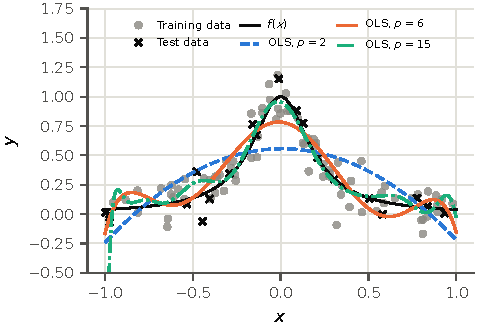
\includegraphics[width=\columnwidth]{a_fits.pdf}
\caption{Runge data and OLS fits on the main 80/20 split. Degree 2 misses much of the central peak, while degree 15 is sensitive near the boundaries. The points marked as test data are not used in fitting.}\label{fig:fits}
\end{figure}

\begin{figure*}[tb]
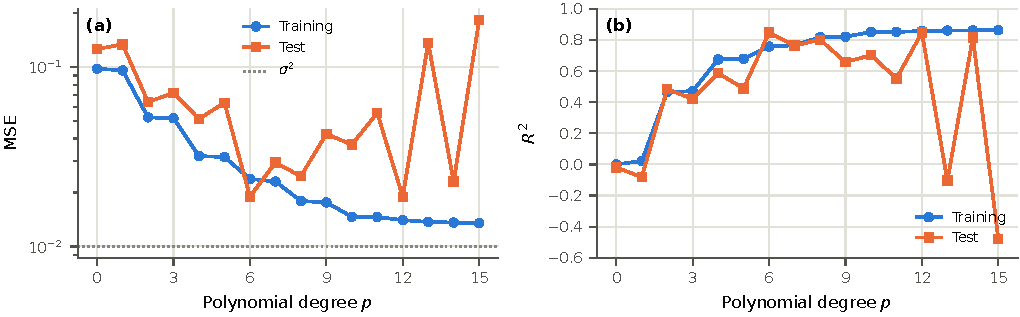
\includegraphics[width=\textwidth]{a_mse_r2.pdf}
\caption{Training and test MSE (left) and $R^2$ (right) versus degree on the main split. Test MSE is 0.01894 at degree 12 and 0.01899 at degree 6; the small difference does not identify a reliable unique optimum. The dotted line in the MSE panel marks the expected noise contribution $\sigma^2=0.01$, not a lower bound on every measured error.}\label{fig:mse_r2}
\end{figure*}

\begin{figure*}[tb]
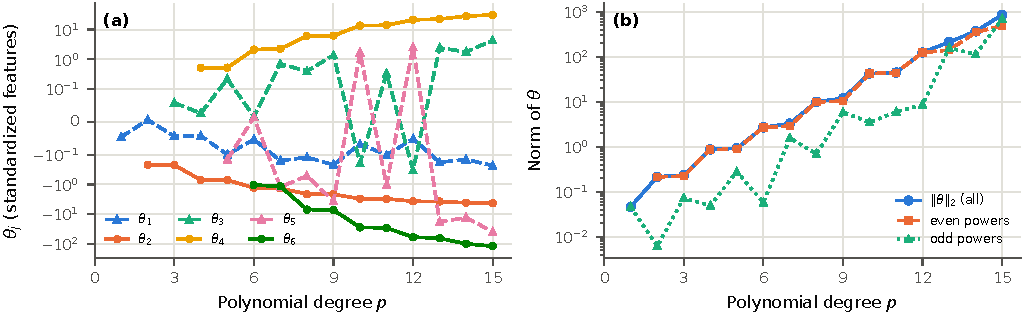
\includegraphics[width=\textwidth]{a_coefficients.pdf}
\caption{Selected standardized coefficients (left) and coefficient norms (right). The norm rises from 2.70 at degree 6 to 856.12 at degree 15. These are slopes in the standardized basis; their magnitudes differ from raw monomial coefficients.}\label{fig:coef}
\end{figure*}

\begin{figure*}[tb]
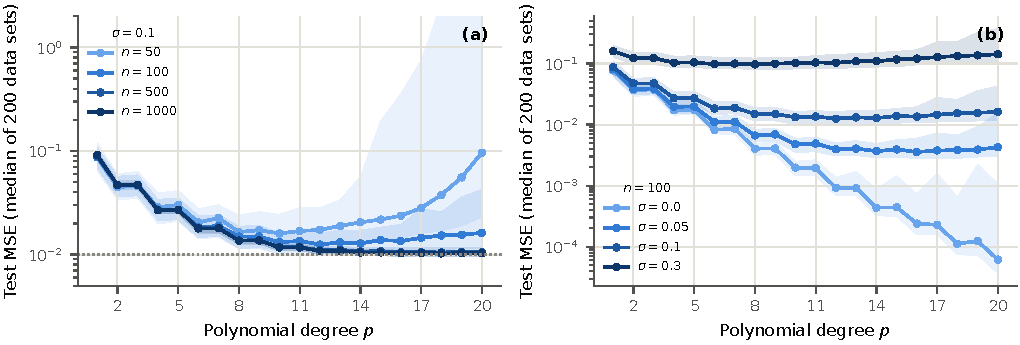
\includegraphics[width=\textwidth]{a_ensemble.pdf}
\caption{OLS test-error medians over 200 datasets for varying total sample size (left) and noise level (right); shading shows interquartile ranges. Larger samples support higher degrees in these median curves, while higher noise favors simpler fits. The dotted line in the left panel marks the noise variance $\sigma^2=0.01$. Medians describe typical outcomes and can conceal rare large errors.}\label{fig:ensemble}
\end{figure*}

\begin{table}[tb]
\caption{Condition number $\kappa(\vX)$ of the design matrix of the main training set for three kinds of preprocessing. ``Raw'' includes a column of ones for the intercept.}\label{tab:scaling}
\begin{ruledtabular}
\begin{tabular}{rccc}
$p$ & raw & centered & standardized \\ \hline
5 & 47.8 & 28.1 & 22.6 \\
10 & $4.1\times10^3$ & $2.6\times10^3$ & $1.6\times10^3$ \\
15 & $4.7\times10^5$ & $3.0\times10^5$ & $1.9\times10^5$ \\
\end{tabular}
\end{ruledtabular}
\end{table}

\subsection{Ridge regression and the singular-value picture}\label{sec:res_ridge}
% Evidence: results/part_b.json/main; code/part_b_ridge.py.
Ridge uses the same main split and degrees 1--20, with 45 logarithmically spaced
penalties from $10^{-10}$ to 10. A logarithmic grid covers weak and strong
shrinkage without concentrating all trials at one scale
\cite[Sec.~3.14]{HjorthJensen2026}. In Fig.~\ref{fig:ridge}, the smallest test MSE
is 0.01347 at degree 10 and $\lambda=1.78\times10^{-6}$, compared with OLS's
0.01894. This grid minimum uses the exploratory test split for selection;
cross-validation and independent evaluation are used for the final comparison.

% Evidence: results/part_b.json/ensemble/best_degree,best_lambda,best_median_mse,
Across 100 new datasets of size 100, Ridge's lowest median MSE is 0.01225 at
degree 12 and $\lambda=5.62\times10^{-8}$; OLS reaches 0.01249 at degree 13.
The improvement in the minimum median is only about $1.9\%$. Repeated datasets
reduce reliance on one favorable split, although 100 repetitions do not reliably
characterize every rare unstable fit. After choosing a penalty separately for
each degree, the Ridge medians remain approximately 0.0123--0.0131 at degrees
12--20. This does not mean that every fixed penalty produces a flat error curve.

% Evidence: results/part_b.json/svd_degree15; Eq.(ridge) and course Sec.3.8.
Figure~\ref{fig:svd} explains the shrinkage using the course SVD formulation
\cite[Sec.~3.8]{HjorthJensen2026}. At degree 15, the singular values range from
27.59 to $1.49\times10^{-4}$. In the last direction, a target projection of
0.1184 becomes an OLS coefficient of 796.24 after division by the singular
value. Its size relative to $\sigma=0.1$ suggests noise sensitivity, without
proving that the projection is entirely noise. Ridge smoothly reduces these
coefficients through $d_j^2/(d_j^2+n\lambda)$. The degree-15 ensemble-selected
penalty gives 12.63 effective slope degrees of freedom; including the
unpenalized intercept gives 13.63.

% Evidence: results/ridge_supplement.json/main and ensemble; code/ridge_supplement.py.
Figures~\ref{fig:ridge_metrics} and \ref{fig:ridge_coefficients} extend the
comparison to training/test MSE, $R^2$ and individual coefficients. Strong
penalties reduce coefficient magnitudes but can leave substantial training and
test error. Figure~\ref{fig:ridge_ensemble} repeats four fixed penalties on
40 paired datasets per sample-size/noise scenario, so each method sees identical
data. The penalties are illustrative settings, not values selected from those
test outcomes. At degree 20 and $\sigma=0.1$, $\lambda=10^{-7}$ reduces median
MSE from 0.2361 to 0.01828 for $N=50$, whereas for $N=1000$ it gives 0.01083
against OLS's 0.01049. With $N=100$ and no noise, the corresponding medians are
0.00101 and 0.0000617. Shrinkage helps some unstable fits but also introduces
bias when little is gained from variance reduction. The spread and heavy tails
limit conclusions from these finite ensembles.

\begin{figure*}[tb]
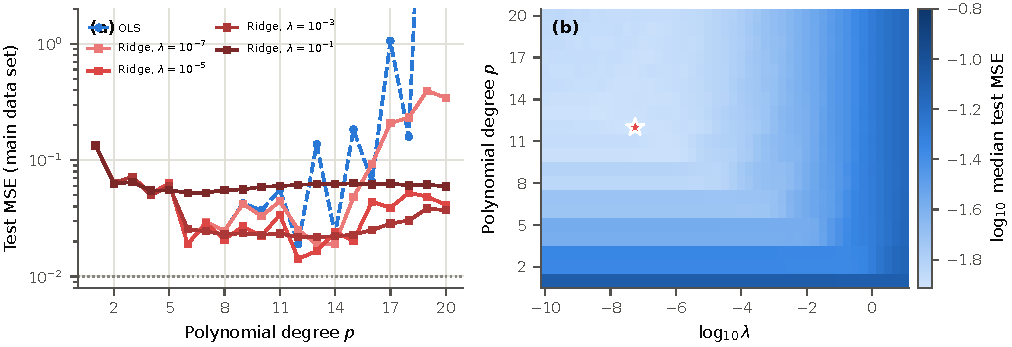
\includegraphics[width=\textwidth]{b_ridge_mse.pdf}
\caption{Ridge test MSE on the main split (left) and median MSE over 100 independent datasets (right). The main-split grid minimum is 0.01347, whereas the ensemble minimum median is 0.01225. The marker identifies the minimum of the displayed grid, not an independently evaluated final model.}\label{fig:ridge}
\end{figure*}

\begin{figure*}[tb]
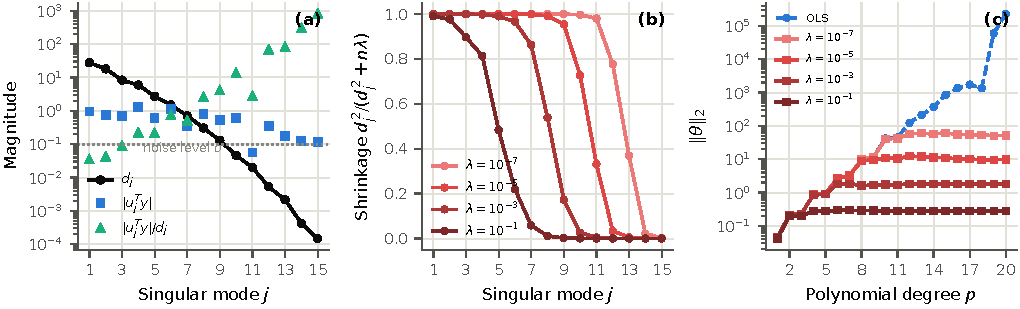
\includegraphics[width=\textwidth]{b_ridge_svd.pdf}
\caption{Degree-15 singular values, target projections and OLS mode coefficients (left); Ridge shrinkage factors (middle); and standardized coefficient norms versus degree (right). Small singular values amplify projections, while increasing the penalty reduces this amplification. Projection size near the dotted noise scale does not prove that a mode contains no signal.}\label{fig:svd}
\end{figure*}

\begin{figure*}[tb]
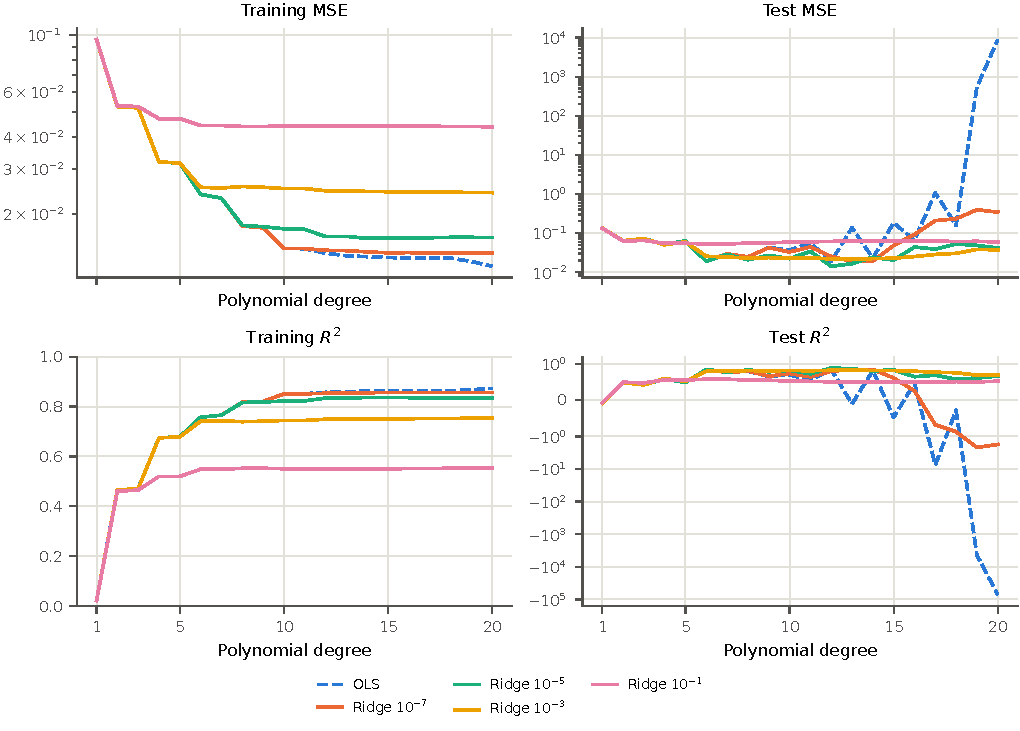
\includegraphics[width=\textwidth]{ridge_supplement_metrics.pdf}
\caption{Training/test MSE and $R^2$ for OLS and four fixed Ridge penalties on the main split, extending the part-a comparison. Training $R^2$ uses a linear axis; test $R^2$ uses a symmetric logarithmic axis to include large negative values. Every score uses the same training or test observations across methods.}\label{fig:ridge_metrics}
\end{figure*}

\begin{figure*}[tb]
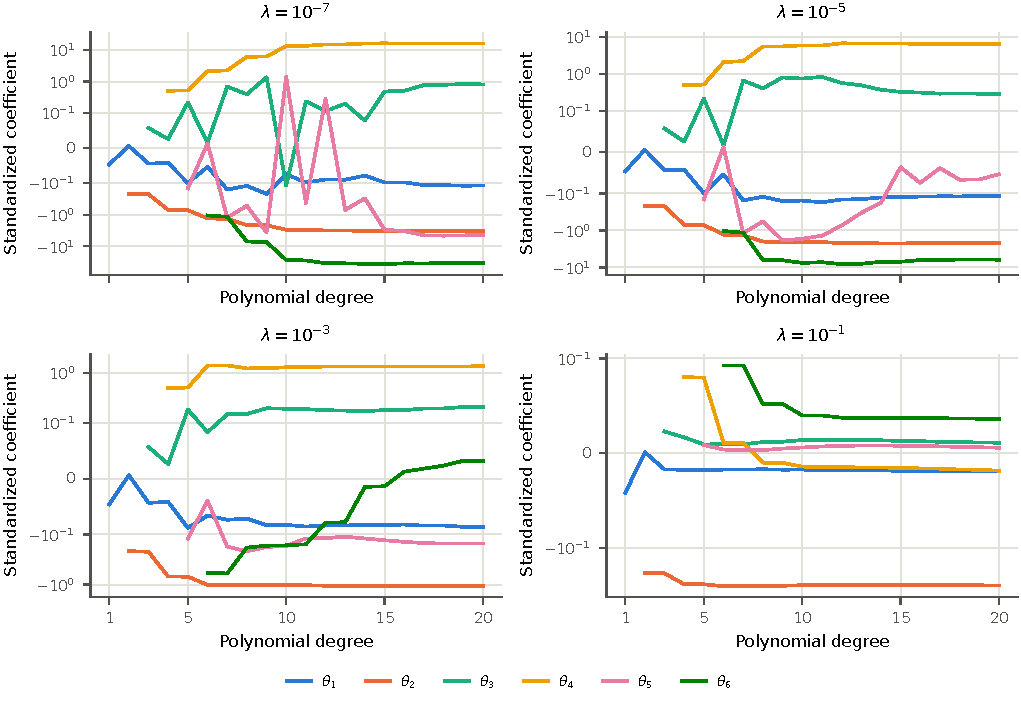
\includegraphics[width=\textwidth]{ridge_supplement_coefficients.pdf}
\caption{The first six standardized Ridge coefficients versus degree at four fixed penalties. Stronger penalties reduce large coefficients, but do not ensure the smallest prediction error. Each panel uses a symmetric logarithmic vertical axis.}\label{fig:ridge_coefficients}
\end{figure*}

\subsection{Training versus test error and the bias--variance trade-off}\label{sec:res_biasvar}
% Evidence: results/part_c.json/train_test; code/part_c_bias_variance.py, R=100,n_train=80.
Following the training/test comparison in the weekly exercises
\cite[Week~35, Exercise~3]{HjorthJensen2026exercises}, Fig.~\ref{fig:hastie}
uses 100 independent training datasets of 80 observations and a fixed independent
test set of 2000 noisy observations. The larger test set reduces the influence
of individual test points. Mean training MSE falls from 0.09106 at degree 0 to
0.00751 at degree 20. Mean test MSE is lowest at degree 8, at 0.01656, whereas
median test MSE is lowest at degree 12, at 0.01339. At degree 12 the mean is
already 0.06142, so a typical fit and average squared-error risk favor different
complexities. Training error below $\sigma^2$ is not itself evidence of leakage:
the training observations were used to fit the model.

% Evidence: code/part_c_bias_variance.py/analyse; results/part_c.json/n=100,n=1000.
The bootstrap calculation follows Week~36 Exercise~3
\cite[Week~36, Exercise~3]{HjorthJensen2026exercises}, with 200 resamples at each
degree and training-only preprocessing. Figure~\ref{fig:biasvar} compares total
sample sizes 100 and 1000, giving 80 and 800 training points. A separate reference
uses 400 fresh training sets of the corresponding size, evaluated at the same
test inputs. The repetition counts balance computation against sampling
variation; they are finite approximations, rather than exact expectations.

% Evidence: results/part_c.json/n=100/best_degree,best_degree_mc,variance[8],variance_mc[8];
With 80 training observations, bootstrap error selects degree 4 while the
fresh-set reference selects degree 8. At degree 8, bootstrap variance is 7.754
against 0.00597 from fresh sets. Resampling the limited training support can
omit boundary observations and make high-degree extrapolation unstable.
An 80-draw bootstrap contains about 50.75 distinct observations on average,
but this fact alone does not imply that bootstrap always overestimates variance.
With 800 training observations, degree-12 variances are much closer:
$1.79\times10^{-4}$ and $1.81\times10^{-4}$. The selected degrees still differ,
18 versus 20, and the empirical bootstrap distribution is not identical to the
population generating fresh data.

% Evidence: results/part_c.json/n=1000/bias2[12],bias2_true[12]; resampling.py.
The noisy-target bias must be interpreted using the derivation in
Sec.~\ref{sec:biasvar_theory}. For $N=1000$ at degree 12, the difference between
squared bias measured against $y$ and against $f$ is 0.01030, close to
$\sigma^2=0.01$. It need not equal 0.01 on a fixed noisy test set because the
realized noise and residual cross term also enter. The numerical identity
error$=$bias$_y^2+$variance is algebraic; it verifies the decomposition of the
stored predictions, not the statistical accuracy of the bootstrap.

\begin{figure}[tb]
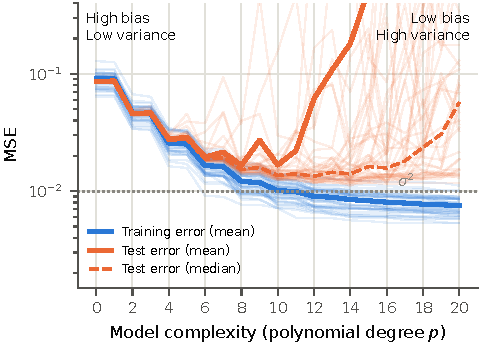
\includegraphics[width=\columnwidth]{c_train_test.pdf}
\caption{Training and test errors from 100 independent 80-observation training sets, evaluated on 2000 fixed fresh noisy test observations. Thin curves show 40 individual runs; thick curves summarize all 100. Mean test error selects degree 8 while median error selects degree 12. The vertical range clips some large errors, including the degree-20 mean of 53.33.}\label{fig:hastie}
\end{figure}

\begin{figure*}[tb]
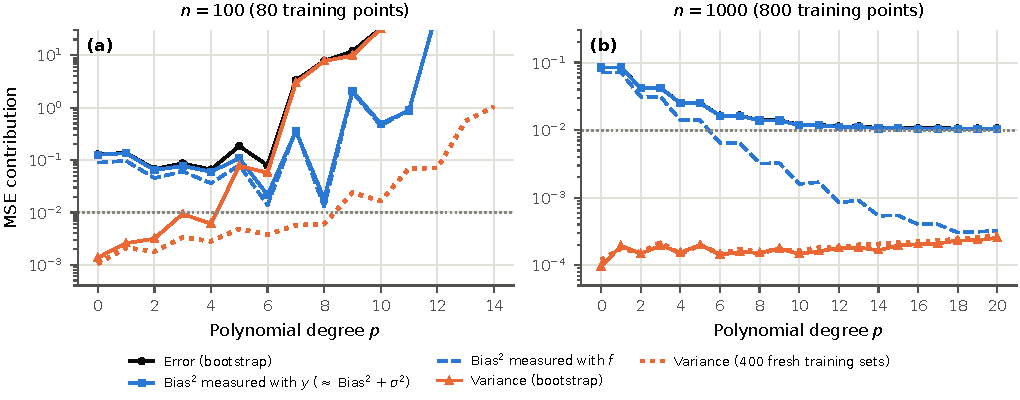
\includegraphics[width=\textwidth]{c_bias_variance.pdf}
\caption{Bootstrap error, noisy-target and true-function squared-bias estimates, and variance for total sample sizes 100 and 1000. Each degree uses 200 bootstrap fits; the dotted variance reference uses 400 fresh training sets. Bias measured against noisy $y$ includes the noise contribution only in expectation. The small-data panel displays degrees through 14 and clips larger values; full arrays are retained in the results files.}\label{fig:biasvar}
\end{figure*}

\subsection{Cross-validation}\label{sec:res_cv}
% Evidence: code/part_d_cross_validation.py; results/part_d.json/ols,ridge.
Five- and tenfold cross-validation use all 100 original observations, giving
80 and 90 training observations per fold. The scaler is fitted inside every
training fold, following the course pipeline
\cite[Secs.~2.12 and 3.14]{HjorthJensen2026}. Both OLS searches select degree 12:
MSE is 0.02016 for fivefold and 0.01731 for tenfold. The one-standard-error
heuristic also selects degree 12. For Ridge, the 21-penalty grid $10^{-10}$--1
selects degree 11 with $\lambda=10^{-6}$ in fivefold CV, giving 0.01788. Tenfold
CV selects degree 12 at the smallest penalty, $10^{-10}$, with MSE 0.017315.
It is effectively unregularized here; the endpoint is not evidence for a uniquely
optimal positive penalty. Figure~\ref{fig:cv} displays the comparison.

% Evidence: results/part_d.json/own_vs_sklearn,ols_svd_relative_cutoff;
The library OLS comparison explicitly uses a relative singular-value cutoff of
$10^{-15}$ to match the pseudoinverse. Scikit-Learn 1.9's default $10^{-6}$
would discard some high-degree directions. With matched cutoffs, the custom
fold scores agree to within $1.18\times10^{-9}$ relatively, including degree 20.
The degree-12 selections are unchanged, but degree-20 CV MSE is 1782.36 for
fivefold and 7.977 for tenfold. These large values lie above the figure's
restricted vertical range.

% Evidence: results/part_d.json/reshuffle,leakage; Sec.3.14 fold-SE qualification.
Across 20 fold reshuffles, selected OLS degrees range from 4--13 for fivefold
and 10--13 for tenfold, with median 12 in both cases. Fold-based error bars are
descriptive because training folds overlap \cite[Sec.~3.14]{HjorthJensen2026}.
Global scaling leaves the checked OLS score unchanged to rounding, but changes
Ridge scores by up to about $0.93\%$ in magnitude. Its small effect here does
not justify fitting preprocessing on held-out inputs.

% Evidence: results/part_c.json/n=100/best_degree; train_test/best_degree_mean,
Bootstrap and CV therefore disagree, selecting degrees 4 and 12. The bootstrap
is particularly pessimistic for this training sample, but CV cannot be declared
exactly correct: fresh-set mean error favors degree 8, while its median favors
12. The methods also use different test observations and, for tenfold CV,
different training sizes. Their curves should be compared with these differences
in mind; independent final evaluation is needed after selecting a model.

\begin{figure*}[tb]
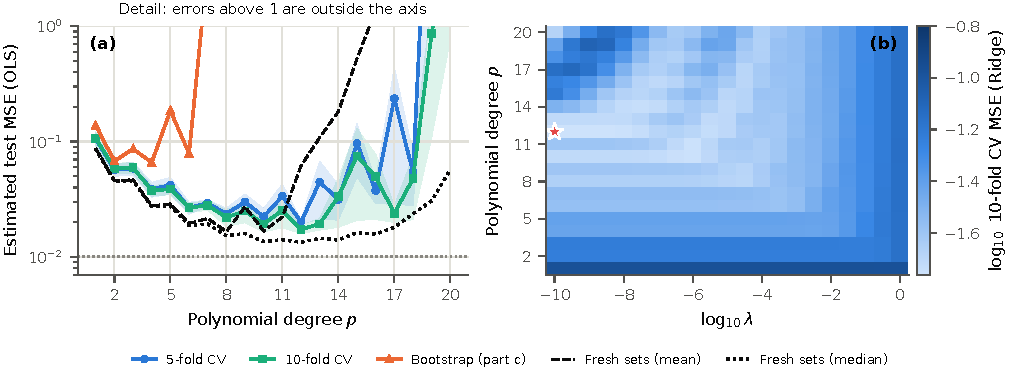
\includegraphics[width=\textwidth]{d_cross_validation.pdf}
\caption{Five- and tenfold OLS CV compared with the fixed-split bootstrap and fresh-training-set mean/median errors (left); tenfold Ridge CV versus degree and penalty (right). Shading shows fold SD divided by $\sqrt{k}$, a descriptive uncertainty measure. The OLS cutoff is $10^{-15}$. The left axis emphasizes errors below 1; degree-20 CV errors of 1782.36 and 7.977 lie outside it. Evaluation samples and training sizes differ between the resampling procedures.}\label{fig:cv}
\end{figure*}

\subsection{Gradient descent with a fixed learning rate}\label{sec:res_gd}
% Evidence: part_e.json.gradient_check; part_e.json.timing; benchmarks.json.gradient_autograd_vs_analytic_max_relative.
The derivative check compares analytical and automatically differentiated gradients at 100 random coefficient vectors for each of degrees 6 and 15. For OLS and Ridge, the largest relative discrepancy is $1.18\times10^{-15}$, consistent with floating-point rounding. Both gradients differentiate the same mean-loss objective, including $2\lambda\vtheta$ for Ridge. The measured AD runtime relative to one cost evaluation falls from 16.1 at $n=80$ to 2.81 at $n=10^6$; implementation overhead matters most for small arrays.

% Evidence: part_e.json.degree6; verification_supplement.json.ridge_gradient_sources and setup.
All convergence comparisons start at zero and use relative coefficient error $\|\vtheta_k-\hat{\vtheta}\|/\|\hat{\vtheta}\|<10^{-6}$. This is a benchmark criterion requiring a reference solution. Table~\ref{tab:gradient_sources} confirms that both derivative sources also agree inside the optimizer, including the supplementary Ridge run.

\begin{table}[tb]
\caption{Degree-6 GD using analytical and AD gradients on the same 80 training observations. Rates minimize worst-case quadratic contraction. The last column compares the final coefficient vectors.}\label{tab:gradient_sources}
\begin{ruledtabular}
\footnotesize
\begin{tabular}{lrrc}
Objective & Analytical steps & AD steps & $\max_j|\Delta\theta_j|$ \\ \hline
OLS & 14\,399 & 14\,399 & $4.44\times10^{-15}$ \\
Ridge, $\lambda=10^{-3}$ & 9\,309 & 9\,309 & $3.33\times10^{-16}$ \\
\end{tabular}
\end{ruledtabular}
\end{table}

% Evidence: part_e.json.degree6.[lambda_max,lambda_min,kappa,eta_max,eta_opt,theory_iterations_eta_opt,scan_fraction,scan_measured,scan_theory].
For degree-6 OLS, $h_{\max}=7.69648$, $h_{\min}=0.00368262$, and $\kappa=2089.95$. The stability bound is therefore $\eta<0.259859$, with $\eta_*=0.259735$. Figure~\ref{fig:gd} shows why rate selection matters: small rates progress slowly, whereas $1.002\eta_{\max}$ amplifies the largest-curvature mode. The eigenmode calculation predicts exactly the observed 14\,399 iterations at $\eta_*$, supporting the quadratic analysis in Sec.~\ref{sec:gd_theory} \cite[Sec.~4.5]{HjorthJensen2026}.

% Evidence: part_e.json.degree6.ridge_table; code/part_e_gradient_descent.py:empirical_threshold.
Table~\ref{tab:gd} shows that increasing Ridge's penalty from zero to $0.1$ reduces $\kappa$ from 2090 to 38.8 and the required iterations from 14\,399 to 244. Adding $2\lambda$ to each Hessian eigenvalue improves conditioning, while changing the estimation problem \cite[Secs.~4.4--4.5]{HjorthJensen2026}. The reported boundary slightly above $\eta_{\max}$ tests only 50\,000 iterations with relative error at most one; it is not a revised asymptotic stability limit. Additional conditioning and early-stopping diagnostics appear in Appendix~\ref{app:additional_checks}.

\begin{figure*}[tb]
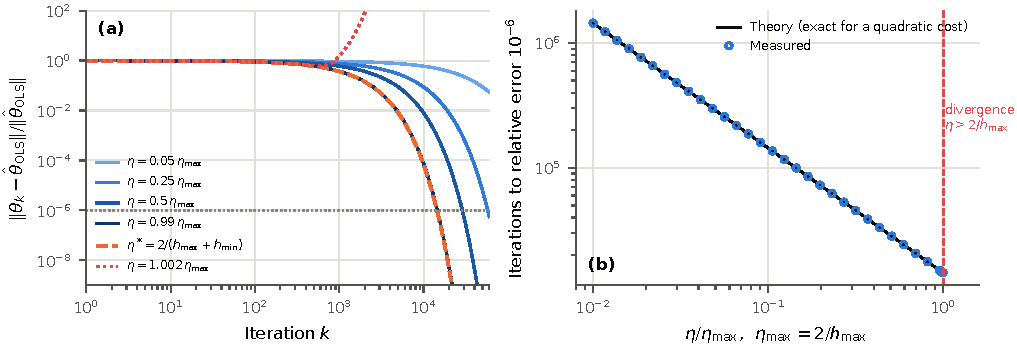
\includegraphics[width=\textwidth]{e_learning_rate.pdf}
\caption{Degree-6 OLS on 80 standardized training observations. (a) Relative coefficient error versus iteration for several fixed rates. (b) Measured iterations to error $10^{-6}$ and the quadratic eigenmode prediction. Rates above $2/h_{\max}$ amplify the highest-curvature mode; very small stable rates converge slowly.}\label{fig:gd}
\end{figure*}

\begin{table}[tb]
\caption{Plain GD at $\eta^*$ for Ridge at $p=6$: smallest Hessian eigenvalue, condition number, and iterations to relative coefficient error $10^{-6}$, matching the eigenmode prediction. The diagnostic $\eta_c$ is the largest tested rate whose relative error remains at most 1 after 50\,000 iterations; it is not an asymptotic stability limit. $h_{\max}$ is 7.70--7.90.}\label{tab:gd}
\begin{ruledtabular}
\begin{tabular}{lcrrc}
$\lambda$ & $h_{\min}$ & $\kappa$ & iterations & $\eta_c/\eta_{\max}$ \\ \hline
0 (OLS) & $3.68\times10^{-3}$ & 2090 & 14\,399 & 1.00004 \\
$10^{-4}$ & $3.88\times10^{-3}$ & 1982 & 13\,655 & 1.00004 \\
$10^{-3}$ & $5.68\times10^{-3}$ & 1355 & 9\,309 & 1.00003 \\
$10^{-2}$ & $2.37\times10^{-2}$ & 326 & 2\,172 & 1.00002 \\
$10^{-1}$ & 0.204 & 39 & 244 & 1.00001 \\
\end{tabular}
\end{ruledtabular}
\end{table}

\subsection{Momentum and adaptive learning rates}\label{sec:res_adaptive}
% Evidence: code/part_f_adaptive.py; part_f.json.degree6.etas and degree6.scan; code/optimizers.py.
The five update rules use identical degree-6 data, analytical gradients and zero initialization. Each method receives the same 28-point rate grid, $10^{-4}$ to $10^{0.5}$, and at most $10^5$ iterations. Rates are compared by steps to relative coefficient error $10^{-6}$, following the comparisons requested in Week~38, Exercises~2--3 \cite{HjorthJensen2026exercises}. Separate tuning is necessary because a rate multiplies differently scaled gradients in the adaptive methods \cite[Secs.~4.8--4.12]{HjorthJensen2026}.

% Evidence: part_f.json.degree6.scan; part_f.json.ridge_degree6.runs.
In Fig.~\ref{fig:optimizers} and Table~\ref{tab:opt}, momentum is fastest on the tested grid: 656 steps at $\eta=0.46416$, against GD's 17\,361. Adam needs 1\,144 steps at its best tested rate and reaches the target at all 28 rates. AdaGrad needs 24\,504 steps; accumulated squared gradients reduce its later step sizes. GD's theoretical optimum is absent from this grid, explaining the larger count than in part e. Reusing the selected rates for Ridge gives 314 steps for momentum and 852 for Adam. These results describe this grid and tolerance, rather than universal rankings.

% Evidence: part_f.json.rmsprop_plateau; part_f.json.rmsprop_decay; part_f.json.degree10.
Constant-rate RMSprop does not attain the target on this grid. After 30\,000 steps its error is $4.54\times10^{-4}$ at $\eta=0.001$ and $4.54\times10^{-3}$ at $0.01$. Scaling by a moving gradient magnitude can maintain appreciable steps near the minimum \cite[Sec.~4.10]{HjorthJensen2026}. Decay reduces the error to $1.50\times10^{-5}$, still above the target. At degree 10, $\kappa=2.70\times10^6$; after 50\,000 steps, the best errors on a separate seven-rate grid are 0.963, 0.763, 0.966, 0.951 and 0.513 for GD, momentum, AdaGrad, RMSprop and Adam. None reaches the target within that budget. Coordinatewise scaling has not removed the difficulty caused by strongly correlated polynomial features.

\begin{figure*}[tb]
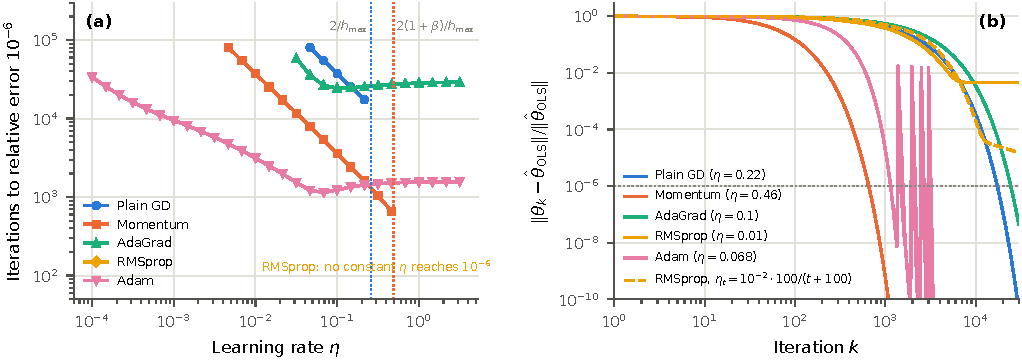
\includegraphics[width=\textwidth]{f_optimizers.pdf}
\caption{Degree-6 OLS optimizer comparison. (a) Steps to relative coefficient error $10^{-6}$ on the tested rate grid, capped at $10^5$ iterations. (b) Histories at each successful method's best grid rate. RMSprop is illustrated at $\eta=0.01$, with and without decay; the decaying run ends at $1.50\times10^{-5}$, above the target.}\label{fig:optimizers}
\end{figure*}

\begin{table}[tb]
\caption{Learning-rate scan at $p=6$: best grid $\eta$ (rounded), iterations to relative coefficient error $10^{-6}$ for OLS and Ridge ($\lambda=10^{-3}$, same $\eta$), successful tested rates within $10^5$ iterations, and best relative error after $5\times10^4$ iterations at $p=10$ ($\kappa=2.7\times10^6$). Dashes mean the target was not attained; the Ridge RMSprop run used $\eta=0.01$. At $\eta^*=0.259735$, absent from the grid, plain GD needs 14\,399 iterations.}\label{tab:opt}
\begin{ruledtabular}
\footnotesize
\setlength{\tabcolsep}{3pt}
\begin{tabular}{lcrrcc}
Method & $\eta$ & OLS & Ridge & converging $\eta$ & $p=10$ \\ \hline
Plain GD & 0.22 & 17\,361 & 11\,217 & 0.046--0.22 & 0.96 \\
Momentum & 0.46 & 656 & 314 & 0.0046--0.46 & 0.76 \\
AdaGrad & 0.10 & 24\,504 & 15\,585 & 0.032--3.2 & 0.97 \\
RMSprop & -- & -- & -- & none & 0.95 \\
Adam & 0.068 & 1\,144 & 852 & $10^{-4}$--3.2 & 0.51 \\
\end{tabular}
\end{ruledtabular}
\end{table}

\subsection{Lasso regression with gradient methods}\label{sec:res_lasso}
% Evidence: part_g.json.autograd_abs_derivative; code/optimizers.py:grad_lasso; Project1.pdf part g; book Secs.3.9,4.14.7.
Autograd returns zero for the derivative convention of $|\theta|$ at zero, and $\pm1$ at $\theta=\pm0.3$. Zero belongs to the subdifferential $[-1,1]$, so it is a valid choice at this nondifferentiable point \cite[Secs.~3.9 and 4.14.7]{HjorthJensen2026}. All custom subgradient runs use $\nabla\MSE+\lambda\,\mathrm{sign}(\vtheta)$, as requested in part g \cite{Project1_2026}. Such updates do not guarantee exact zero coefficients: at a zero coordinate, the data gradient need not itself vanish. The reference is scikit-learn's coordinate-descent Lasso with $\alpha=\lambda/2$, matching our normalization.

% Evidence: lasso_course_comparison.json.setup, selected, reference; code/lasso_course_comparison.py.
To cover all five taught updates, a supplementary comparison uses the same eight rates per method: seven logarithmically spaced values from $10^{-4}$ to $0.1$, plus $1/L$. All runs start at zero and use 40\,000 updates. Each method's rate minimizes its mean training objective gap over the final 200 updates; test MSE does not select it. Table~\ref{tab:lasso-course-methods} shows that Adam achieves the smallest final coefficient error. All five runs retain small nonzero coefficients where the reference has three exact zeros. This is a finite-grid comparison, not a convergence guarantee.

\begin{table}[tb]
\caption{All five course update rules for degree-10 Lasso at $\lambda=10^{-3}$. Values describe the selected run's final iterate; $r$ is relative coefficient error and $\Delta C$ is the penalized objective gap. None produces exact zero coefficients.}\label{tab:lasso-course-methods}
\begin{ruledtabular}
\footnotesize
\begin{tabular}{lccc}
Method & $\eta$ & $\Delta C$ & $r$ \\ \hline
GD & 0.1 & $5.16\times10^{-5}$ & 0.158 \\
Momentum & 0.03162 & $1.61\times10^{-7}$ & 0.00353 \\
AdaGrad & 0.07820 & $7.99\times10^{-5}$ & 0.186 \\
RMSprop & 0.0003162 & $1.70\times10^{-5}$ & 0.0851 \\
Adam & 0.0003162 & $4.98\times10^{-8}$ & $2.98\times10^{-5}$ \\
\end{tabular}
\end{ruledtabular}
\end{table}

% Evidence: part_g.json.convergence, especially Subgradient GD and Subgradient Adam; code/part_g_lasso.py.
In the original plotted comparison at degree 10 and $\lambda=10^{-3}$, 40\,000 subgradient-GD steps at $\eta=1/L=0.07820$ leave objective gap $C(\vtheta)-C(\hat{\vtheta})=1.30\times10^{-4}$. Adam at $\eta=0.01$ reduces this to $7.54\times10^{-6}$. Neither gives exact zeros, although Adam's largest coefficient difference from the reference is only 0.00106. Thus improved numerical accuracy does not automatically reproduce Lasso's exact sparsity.

% Evidence: part_g.json.fista_vs_sklearn; part_g.json.convergence; part_g.json.path; code/part_g_lasso.py:path and check_idx.
Figure~\ref{fig:lasso} includes optional proximal comparisons, ISTA and FISTA \cite{Beck2009}, alongside the required subgradient methods. At 40\,000 steps, ISTA identifies two of the three reference zeros; FISTA identifies all three and reaches objective gap $9.50\times10^{-12}$, although its maximum coefficient error remains $1.47\times10^{-4}$. Flat directions explain why objective and coefficient accuracies differ. Separately, nine FISTA checks along the sklearn coefficient path agree within $2.91\times10^{-8}$ and share its zero pattern. Even terms enter first, at $\lambda=0.3393$, before an odd term at 0.01351. This agrees with the target's symmetry without requiring odd coefficients to vanish in a finite noisy sample.

% Evidence: part_g.json.methods_degree10.rows; lambda_ridge=1e-4, lambda_lasso=1e-3, iterations=10000.
After 10\,000 steps at degree 10, OLS-GD has test MSE 0.01990 versus 0.03702 for exact OLS, despite relative coefficient error 0.990. Incomplete fitting improves prediction on this particular split. For Ridge ($\lambda=10^{-4}$), Adam gives 0.019892 versus the reference 0.019887; for Lasso ($\lambda=10^{-3}$), the corresponding values are 0.019220 and 0.019221. Their remaining coefficient errors are 0.00226 and 0.000435. These comparisons separate optimizer accuracy from generalization; they do not justify selecting a stopping time by repeatedly inspecting test error.

\begin{figure*}[tb]
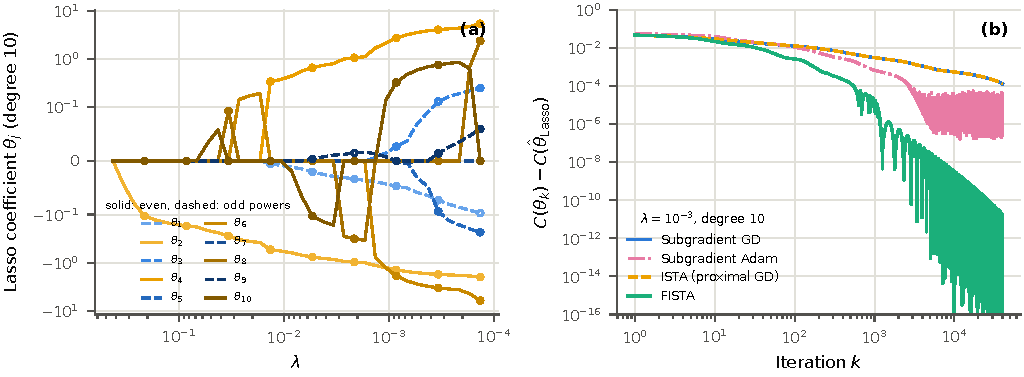
\includegraphics[width=\textwidth]{g_lasso.pdf}
\caption{Degree-10 Lasso. (a) Scikit-learn coordinate-descent paths, with nine custom FISTA checks; solid and dashed lines denote even and odd powers. (b) Excess penalized training cost at $\lambda=10^{-3}$ for custom subgradient GD and Adam, together with optional ISTA/FISTA comparisons. Objective accuracy and exact coefficient sparsity are distinct diagnostics.}\label{fig:lasso}
\end{figure*}

\subsection{Stochastic gradient descent}\label{sec:res_sgd}
% Evidence: code/part_h_sgd.py; part_h.json.setup, batch_size; book4.7.8-4.7.9, Week38Exercise4.
The degree-6 OLS experiment runs 2\,000 epochs with batch sizes $M=1,5,20,80$, reshuffling each epoch as in Week~38, Exercise~4 \cite{HjorthJensen2026exercises}. Constant rates and inverse-time schedules are tuned by the geometric mean excess training cost over the last 200 epochs on shuffle seed zero; the plotted curves summarize five seeds. These seeds vary the optimization order, not the dataset. For the chosen decays, $t_1$ corresponds to 250 epochs. The grids, seeds and iteration budgets are computational choices, not guarantees of optimal tuning. Individual batch gradients can remain nonzero at the full-data optimum, explaining why constant-rate SGD may fluctuate there. Decay reduces these fluctuations but also slows late progress.

% Evidence: part_h.json.batch_size, full_batch_eta_opt; course book4.7.8-4.7.9.
Figure~\ref{fig:sgd}(a) shows that decay improves batch-5 final excess cost from $4.37\times10^{-4}$ to $4.70\times10^{-5}$. Its median curve first crosses $\sigma^2p/n=0.00075$ after 306 epochs. Constant full-batch GD at $\eta=0.25$ crosses after 1\,526 epochs, versus 1\,973 at $\eta_*$. The latter optimizes worst-case coefficient contraction, not this particular cost threshold. The horizontal line is a statistical reference scale, not a strict optimization floor \cite[Secs.~4.7.8--4.7.9]{HjorthJensen2026}. Small excess cost need not imply small coefficient error: $\Delta C=\tfrac12 e^THe$ gives little weight to flat directions. Full-batch decay ends at coefficient error 0.601, showing that decay can also slow progress.

% Evidence: part_h.json.methods_M10; part_h.json.batch_size[1].constant.time_s and batch_size[80].constant.time_s.
For $M=10$, Adam reaches the reference scale first, at 725 epochs, and ends with coefficient error 0.0204. Its runtime is 0.230~s, compared with 0.117~s for plain SGD. Across batch sizes, 2\,000 epochs process the same 160\,000 sample contributions, but $M=1$ performs 160\,000 updates and $M=80$ only 2\,000. Their constant-rate runtimes are 0.871 and 0.0454~s. Smaller batches reduce work per update but increase update overhead; epochs alone are not a runtime comparison.

% Evidence: verification_supplement.json.setup; ridge_sgd_methods_M10; ridge_full_batch_gd_eta_opt; ridge_full_batch_sgd_vs_gd_max_abs.
The supplementary Ridge comparison uses $\lambda=10^{-3}$, a nine-rate grid per method, and three shuffle seeds (Table~\ref{tab:ridge_sgd}). Adam gives greater accuracy than 2\,000 full-batch updates, but takes more time. Adding decay with the same initial rate, without retuning, worsens the finite-budget coefficient errors. This does not establish that every decaying schedule is inferior. Full-batch Ridge SGD matches ordinary GD within $2.22\times10^{-16}$, checking the shared update logic. For these small matrices, the closed-form SVD remains a practical reference; the experiment does not demonstrate a large-data SGD speedup.

\begin{table}[tb]
\caption{Supplementary degree-6 Ridge optimization after 2\,000 epochs. SGD uses $M=10$; entries are medians over three shuffle seeds. $r$ is relative coefficient error and $\Delta C$ includes the Ridge penalty. Full GD uses $\eta_*=0.259600$.}\label{tab:ridge_sgd}
\begin{ruledtabular}
\footnotesize
\begin{tabular}{lcccc}
Method & $\eta$ & $r$ & $\Delta C$ & Time (s) \\ \hline
SGD & 0.03162 & 0.0485 & $8.72\times10^{-5}$ & 0.153 \\
Momentum & 0.003162 & 0.0510 & $3.52\times10^{-5}$ & 0.186 \\
AdaGrad & 0.3162 & 0.0207 & $6.55\times10^{-5}$ & 0.200 \\
RMSprop & 0.003162 & 0.0218 & $2.22\times10^{-4}$ & 0.202 \\
Adam & 0.003162 & 0.0185 & $8.91\times10^{-6}$ & 0.297 \\
Full GD & 0.259600 & 0.0485 & $7.71\times10^{-5}$ & 0.0528 \\
\end{tabular}
\end{ruledtabular}
\end{table}

\begin{figure*}[tb]
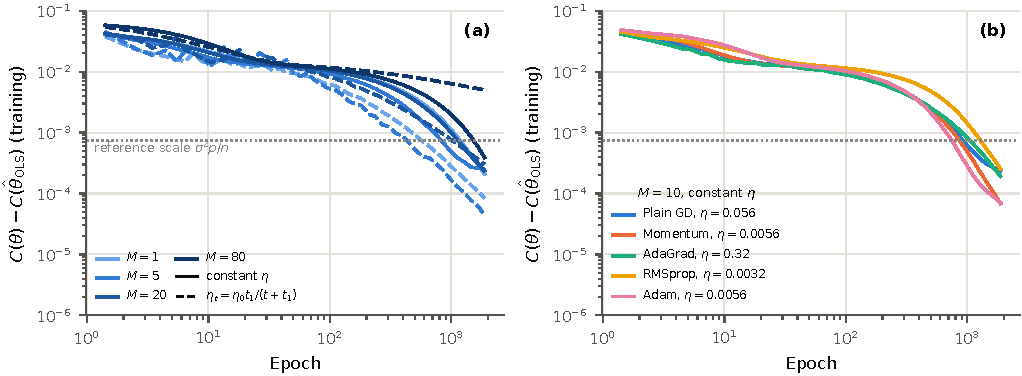
\includegraphics[width=\textwidth]{h_sgd.pdf}
\caption{Mini-batch degree-6 OLS on 80 training observations. (a) Batch sizes 1, 5, 20 and 80 with separately tuned constant and inverse-time schedules. (b) Five update rules at batch size 10. Curves summarize five shuffle seeds and are smoothed in logarithmic epoch bins. Epochs count data passes; $\sigma^2p/n$ is a statistical reference scale.}\label{fig:sgd}
\end{figure*}

\subsection{Final model selection}\label{sec:res_final}
% Evidence: results/part_i.json: grids, sigma=0.1, sigma=0.3.
Ten-fold CV compares all three estimators on the same 100 observations and fold assignments. Degrees range from 1 to 20. Ridge uses 21 logarithmically spaced penalties from $10^{-10}$ to 1; Lasso uses seven from $10^{-4}$ to $10^{-1}$. A logarithmic grid covers several penalty scales without requiring an excessively large search. The larger lower bound for Lasso is a computational restriction: very small penalties and correlated high-degree columns make coordinate descent slow. It is not evidence that smaller penalties could never be useful. The selection procedure follows the course CV workflow \cite[Sec.~3.14]{HjorthJensen2026}; the stated complexity measure defines its additional one-SE choices.

Each selected model is refitted on all 100 observations and evaluated on 2000 independently generated observations with seed 2027. This larger test set reduces evaluation noise compared with the original 20-point holdout, although its MSE remains a finite estimate. It is used after selection, not to choose a second winner. Table~\ref{tab:final} reports both minimum-CV and one-SE models.

At $\sigma=0.1$, the lowest CV score is OLS at degree 12. Ridge chooses degree 12 and its smallest penalty, giving almost the same fit. Their CV scores differ by about $1.8\times10^{-6}$, much less than the descriptive fold SE of about 0.00137. There is little practical reason to prefer that nearly unregularized Ridge model to OLS. The OLS independent-test MSE is 0.0113, about 13\% above the noise contribution 0.01. Lasso's minimum has ten nonzero slopes at degree 15 and test MSE 0.01325. Five retained powers are odd and five even: the population symmetry does not force exact symmetry in a noisy, randomly sampled fit.

At $\sigma=0.3$, Ridge has the lowest CV MSE, 0.14125, followed by Lasso at 0.14223 and OLS at 0.14538. These differences are small compared with fold SEs around 0.013--0.014. The independent-test MSEs, 0.09758, 0.09907 and 0.09766, are likewise close. The one-SE choices use fewer effective slopes or nonzero terms. For Ridge, effective slope df falls from 9.61 to 4.92 while test MSE increases by about 6.9\%. This is an explicit trade-off between simplicity and observed prediction accuracy, not proof that the simpler model has the same population risk.

CV errors exceed the final test errors in this realization. Each CV model trains on 90 observations, while the refit uses 100, but this does not explain the entire difference. Fold locations, realized noise, selection over several candidates and the different test sample also matter. A single experiment cannot isolate their contributions.

% Evidence: results/part_i.json: bias_variance_degree15; 150 fresh sets and 150 bootstrap draws.
Figure~\ref{fig:final}(b,c) studies regularization at degree 15 using 150 independent training sets of 80 observations and 150 bootstrap resamples. Both are evaluated against the known function on 401 equally spaced inputs. The repeat count balances computation and the need to see variation between fits; it does not guarantee a stable estimate of rare large errors. For OLS, estimated squared bias is 0.00654 and variance is 0.21098. At the lowest sampled fresh-set risk, Ridge with $\lambda=3.16\times10^{-4}$ gives squared bias 0.00670 and variance 0.00349. Lasso at the same penalty gives 0.00487 and 0.00363. Ridge therefore reduces this variance estimate by about a factor of 60, with a small increase in squared bias. Lasso also reduces variance strongly. These penalties use known-function risk and are explanatory choices, distinct from the CV selections.

The bootstrap variance for degree-15 OLS is about $9.05\times10^4$ in this experiment. That extreme conditional estimate reflects unstable resampled boundary support; it should not be presented as a precise population variance. The evidence across parts b and i supports regularization mainly as protection against high-degree instability here, rather than a guarantee of lower error than a carefully selected OLS degree.

% Evidence: results/part_i.json: lasso_convergence_cv; results/model_selection_check.json.
Solver accuracy is another limitation. In the original search, 338 of 3080 Lasso model-selection fits reached the iteration limit; this includes fold fits and full-data refits. Refining the four reported Lasso choices to tolerance $10^{-10}$ changed their CV scores by at most 0.045\%, with KKT residuals below $7.1\times10^{-11}$. Their reported scores are thus insensitive to this stricter solve, but the whole candidate grid has not been reranked at that tolerance.

\begin{table*}[tb]
\caption{Models selected by 10-fold cross-validation on $n=100$ observations at two noise levels, using minimum CV error (min) or the one-standard-error heuristic (1SE). Test MSE on 2000 independent noisy observations estimates prediction risk; the noise variances are $\sigma^2=0.01$ and 0.09. CV uncertainties are fold-based standard errors. ``Size'' counts slopes only: degree for OLS, nonzero slopes for Lasso, and effective slope degrees of freedom for Ridge; the unpenalized intercept is excluded.}\label{tab:final}
\begin{ruledtabular}
\begin{tabular}{llcccccc}
$\sigma$ & Method & Rule & $p$ & $\lambda$ & CV MSE & Independent test MSE & Size \\ \hline
0.1 & OLS & min = 1SE & 12 & -- & $0.0173\pm0.0014$ & 0.0113 & 12 \\
0.1 & Ridge & min & 12 & $10^{-10}$ & $0.0173\pm0.0014$ & 0.0113 & df = 12.0 \\
0.1 & Ridge & 1SE & 10 & $10^{-6}$ & $0.0176\pm0.0022$ & 0.0124 & df = 9.6 \\
0.1 & Lasso & min & 15 & $10^{-4}$ & $0.0192\pm0.0024$ & 0.0132 & 10 \\
0.1 & Lasso & 1SE & 8 & $10^{-4}$ & $0.0207\pm0.0028$ & 0.0143 & 8 \\[2pt]
0.3 & OLS & min & 10 & -- & $0.145\pm0.013$ & 0.0977 & 10 \\
0.3 & OLS & 1SE & 4 & -- & $0.157\pm0.017$ & 0.1078 & 4 \\
0.3 & Ridge & min & 10 & $10^{-6}$ & $0.141\pm0.013$ & 0.0976 & df = 9.6 \\
0.3 & Ridge & 1SE & 6 & $3.2\times10^{-3}$ & $0.152\pm0.017$ & 0.1043 & df = 4.9 \\
0.3 & Lasso & min & 8 & $3.2\times10^{-4}$ & $0.142\pm0.014$ & 0.0991 & 8 \\
0.3 & Lasso & 1SE & 4 & $3.2\times10^{-3}$ & $0.157\pm0.018$ & 0.1073 & 4 \\
\end{tabular}
\end{ruledtabular}
\end{table*}

\begin{figure*}[tb]
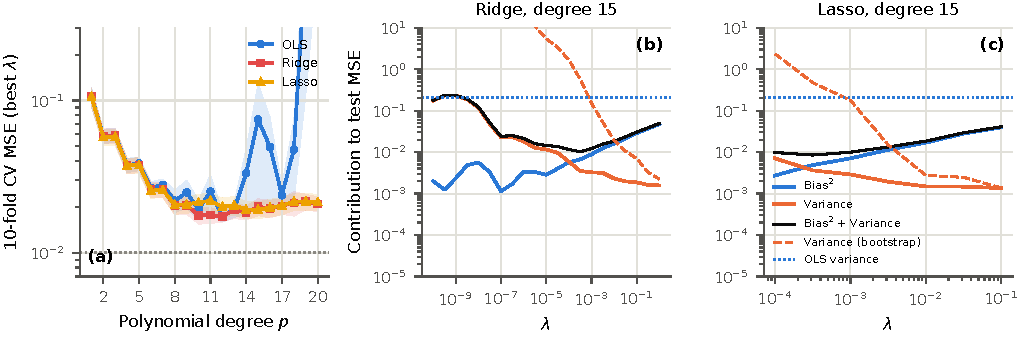
\includegraphics[width=\textwidth]{i_model_selection.pdf}
\caption{Final model comparison. (a) Ten-fold CV MSE at each degree, minimized over the tested penalties; bands show descriptive fold SEs, and the dotted line marks $\sigma^2=0.01$. Values above the displayed range are omitted from the axis. (b,c) Degree-15 bias and variance estimates versus Ridge/Lasso penalty, using 150 independent 80-point training sets and 150 bootstrap samples. Predictions are evaluated against the known function at 401 fixed inputs. Bias$^2$ plus variance excludes the additional test-noise term. The OLS variance is shown for comparison; bootstrap and independent-set curves estimate different training distributions.}\label{fig:final}
\end{figure*}

\section{Conclusions}\label{sec:conclusion}
\emph{LLM contribution: this section was drafted with assistance; see Appendix~\ref{app:llm}.}

The Runge experiment shows that increasing polynomial degree helps only while the extra flexibility is supported by the data. On the main split, degrees 6 and 12 have almost equal test errors, while higher degrees can produce large boundary errors. More observations reduce this instability. At noise SD 0.1, minimum ten-fold CV selects degree-12 OLS, and nearly unpenalized Ridge gives essentially the same result. Ridge and Lasso are most useful here for stabilizing the wider range of high-degree models. At the higher noise level the selected models are less complex, although the observed differences between estimators remain small.

Resampling and optimization answer different questions. The small-sample bootstrap can lose boundary support, so its error and variance estimates need not agree with independent-training-set estimates or CV. Mean and median errors also differ when rare fits are very inaccurate. For optimization, analytical and automatic gradients agree to rounding precision in the tested cases. Learning-rate choice and conditioning strongly affect convergence. Momentum performs well on the degree-six problem, but no optimizer wins at every budget and degree. Smaller SGD batches provide more updates per data pass, while their extra overhead can make them slower in wall time.

The conclusions are limited to the tested function, distributions, grids and budgets. The 20-point exploratory holdout is too small to establish a precise model ranking, and the original Lasso grid contains unfinished fits. Repeated outer validation would give a clearer assessment of model-selection variability. An even polynomial basis would test whether using the known symmetry reduces unnecessary parameters; an orthogonal basis would help separate monomial conditioning from statistical difficulty. Larger independent ensembles could better describe the tails of the error distribution, and measuring time to a common accuracy target would improve the optimizer comparison. These are proposed extensions, not experiments claimed in this report.

\appendix
\section{Use of AI/LLM tools}\label{app:llm}
\paragraph{Tools and contributions.}
The original code and report structure are attributed in the project files to Claude through
Claude Code, October 2026. The precise original model label has not been independently verified.
OpenAI Codex was used through the Codex desktop app on October 5, 2026 to inspect the course
material and code, audit numerical claims, run verification, add supplementary experiments,
and generate this report draft and its writing guide. The course declaration guidelines provide the contribution
levels used below \cite{LLMGuidelines2026}.

\paragraph{Text.}
The prompts requested worked answers to parts a--i, explanations of each choice, connections
to lectures and exercises, and a complete report using straightforward language.
The draft was revised during the session to correct penalty normalization and intercept
wording, qualify resampling and convergence claims, separate extra algorithms, and connect
numerical claims to saved results. Theory, interpretations, captions and the report prose
were generated or substantially revised by Codex. The original equations and layout also had Claude assistance.

\begin{table}[tb]
\caption{Text contributions in this draft, using the course's levels 0--3.}
\label{tab:llm_text}
\begin{ruledtabular}
\small
\begin{tabular}{lc}
Section & Level \\ \hline
Abstract & 3 \\
Introduction & 3 \\
Theory and methods & 3 \\
Implementation and verification & 3 \\
Results and discussion & 3 \\
Conclusions & 3 \\
Appendices and captions & 3 \\
\end{tabular}
\end{ruledtabular}
\end{table}

\paragraph{Code and verification.}
The original numerical modules, task scripts, helpers and tests have substantial generated
code contributions. Codex corrected the OLS reference rank tolerance in part d and related
checks, added a high-degree regression test, and improved course-linked documentation.
The supplementary scripts were generated by Codex. Function-level assistance tags record
these contributions. Table~\ref{tab:llm_code} groups files with the same origin; individual
filenames and execution commands are listed in the README.

The recorded 26-test run, benchmark reproduction, part-d rerun and supplementary experiments
were executed by Codex. The author's own review is not recorded by these automated checks.

\begin{table}[tb]
\caption{Code contributions using the course's levels 0--4.}
\label{tab:llm_code}
\begin{ruledtabular}
\small
\begin{tabular}{p{0.50\columnwidth}cp{0.32\columnwidth}}
Files & Level & Contribution \\ \hline
\texttt{regression.py}, \texttt{resampling.py}, \texttt{optimizers.py}
& 4 & Claude implementation; Codex documentation and audit \\
\texttt{part\_*.py}, \texttt{benchmarks.py}
& 4 & Claude implementation; Codex targeted corrections \\
\texttt{settings.py}, \texttt{plot\_style.py}, \texttt{run\_all.py}
& 4 & Claude implementation \\
\texttt{tests/}
& 4 & Original generated tests; Codex rank-cutoff check \\
Supplementary scripts
& 4 & Codex implementation and execution \\
\end{tabular}
\end{ruledtabular}
\end{table}

\section{Additional conditioning and stopping diagnostics}\label{app:additional_checks}
The conditioning experiment in Fig.~\ref{fig:kappa}(a) builds on the course's Hessian and
momentum analysis \cite[Secs.~4.5--4.6]{HjorthJensen2026}. The extra heavy-ball comparison
chooses both parameters from the Hessian spectrum; these settings are additional to the
fixed-momentum runs used for the main comparison. Specifically,
$\eta=4/(\sqrt{h_{\max}}+\sqrt{h_{\min}})^2$ and
$\beta=((\sqrt{\kappa}-1)/(\sqrt{\kappa}+1))^2$.
Early stopping itself is discussed in
\cite[Sec.~4.7.8]{HjorthJensen2026}. Panel (b) extends that idea with an explicit spectral
comparison to Ridge and a known-function diagnostic, separately from the required
fixed-rate convergence experiment.

For unregularized GD initialized at zero, write $h_i$ for the eigenvalues of $2\vX^T\vX/n$
and $\bm v_i$ for the associated eigenvectors. Applying the error recurrence in
Eq.~(\ref{eq:gd_modes}) gives
\begin{align}
\vtheta_k
&=\sum_i\big[1-(1-\eta h_i)^k\big]
 (\bm v_i^T\hat{\vtheta}_{\rm OLS})\,\bm v_i,\nonumber\\
\lambda_{\rm eff}&\approx\frac{1}{2\eta k}. \label{eq:gd_filter}
\end{align}
The effective penalty compares the small-eigenvalue slopes of the GD filter and the Ridge
filter $h_i/(h_i+2\lambda)$; the two estimators are not identical.
Early stopping as regularization is discussed in \cite{Ali2019}.
The present experiment evaluates a dense grid using the known function and adds $\sigma^2$.
Selecting the best checkpoint from that grid is an oracle diagnostic, not a validation rule
available when the true function is unknown.

\begin{figure*}[tb]
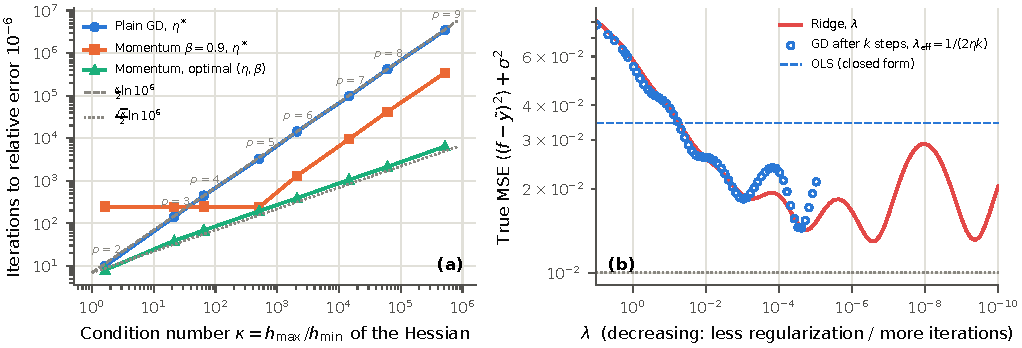
\includegraphics[width=\textwidth]{e_kappa.pdf}
\caption{Additional diagnostics. (a) Iteration counts versus Hessian conditioning, including
fixed-momentum and Hessian-tuned heavy-ball updates. (b) Degree-15 GD checkpoints and Ridge
evaluated on a known-function grid, with test-noise variance added. The effective-penalty
axis compares scales rather than equating the estimators. The best plotted values use the
known function and are not independently selected test results.}\label{fig:kappa}
\end{figure*}

\section{Additional Ridge diagnostics}\label{app:ridge_extra}
The fixed-penalty Ridge comparisons in Fig.~\ref{fig:ridge_ensemble} use the same
datasets for every estimator in a repetition. This isolates the effect of the penalty
from variation between data draws. The curves supplement the sample-size and noise
comparison in Sec.~\ref{sec:res_ridge}.

\begin{figure*}[tb]
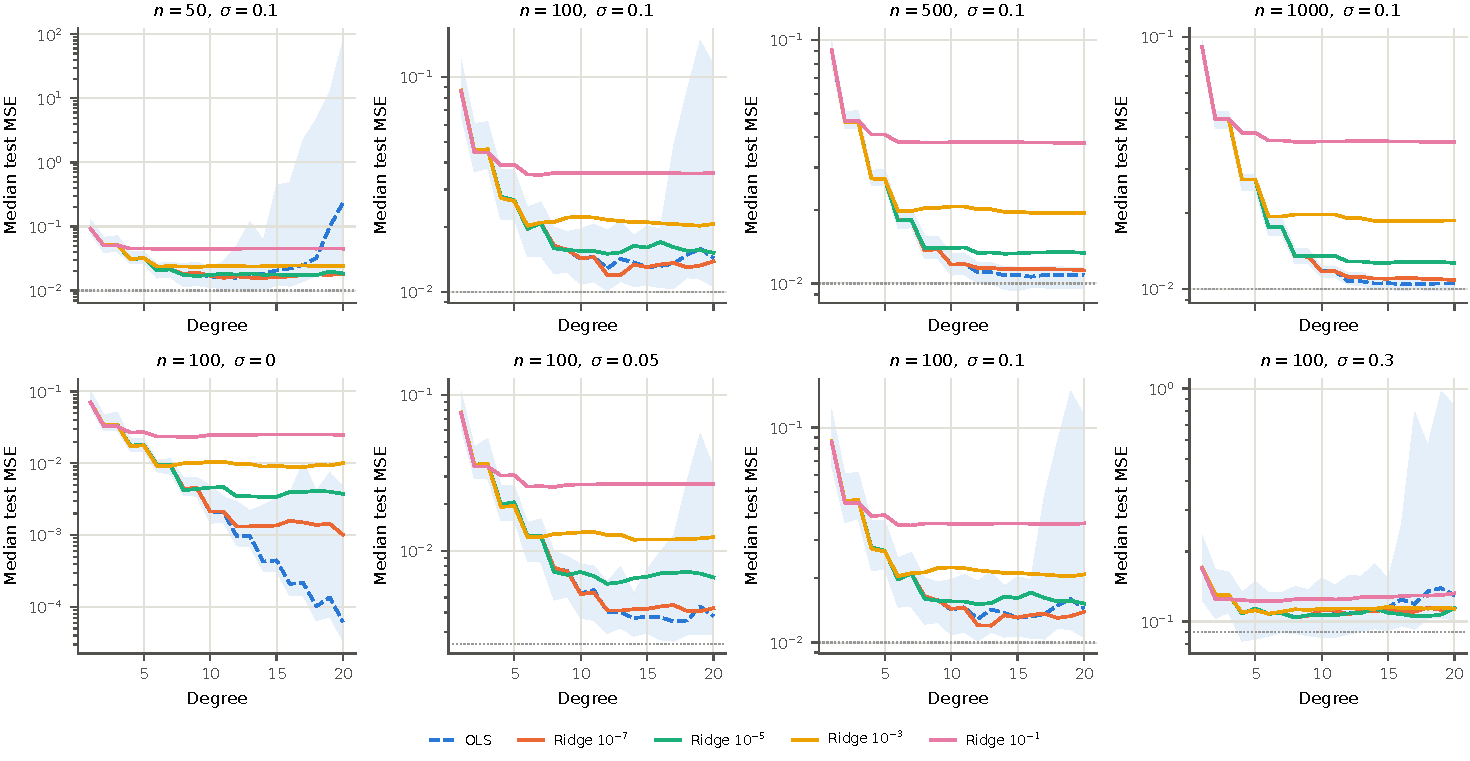
\includegraphics[width=\textwidth]{ridge_supplement_ensemble.pdf}
\caption{Median test MSE for OLS and fixed Ridge penalties over 40 paired datasets per scenario. Top row: varying total sample size at $\sigma=0.1$; bottom row: varying noise at $N=100$. OLS shading shows its interquartile range; dotted lines mark $\sigma^2$ when nonzero. These fixed-penalty comparisons do not select hyperparameters using the test outcomes.}\label{fig:ridge_ensemble}
\end{figure*}

\bibliography{references}

\end{document}
